% Options for packages loaded elsewhere
\PassOptionsToPackage{unicode}{hyperref}
\PassOptionsToPackage{hyphens}{url}
\PassOptionsToPackage{dvipsnames,svgnames*,x11names*}{xcolor}
%
\documentclass[
]{krantz}
\usepackage{lmodern}
\usepackage{amssymb,amsmath}
\usepackage{ifxetex,ifluatex}
\ifnum 0\ifxetex 1\fi\ifluatex 1\fi=0 % if pdftex
  \usepackage[T1]{fontenc}
  \usepackage[utf8]{inputenc}
  \usepackage{textcomp} % provide euro and other symbols
\else % if luatex or xetex
  \usepackage{unicode-math}
  \defaultfontfeatures{Scale=MatchLowercase}
  \defaultfontfeatures[\rmfamily]{Ligatures=TeX,Scale=1}
\fi
% Use upquote if available, for straight quotes in verbatim environments
\IfFileExists{upquote.sty}{\usepackage{upquote}}{}
\IfFileExists{microtype.sty}{% use microtype if available
  \usepackage[]{microtype}
  \UseMicrotypeSet[protrusion]{basicmath} % disable protrusion for tt fonts
}{}
\makeatletter
\@ifundefined{KOMAClassName}{% if non-KOMA class
  \IfFileExists{parskip.sty}{%
    \usepackage{parskip}
  }{% else
    \setlength{\parindent}{0pt}
    \setlength{\parskip}{6pt plus 2pt minus 1pt}}
}{% if KOMA class
  \KOMAoptions{parskip=half}}
\makeatother
\usepackage{xcolor}
\IfFileExists{xurl.sty}{\usepackage{xurl}}{} % add URL line breaks if available
\IfFileExists{bookmark.sty}{\usepackage{bookmark}}{\usepackage{hyperref}}
\hypersetup{
  pdftitle={Broadening Your Statistical Horizons},
  pdfauthor={Julie Legler and Paul Roback},
  colorlinks=true,
  linkcolor=Maroon,
  filecolor=Maroon,
  citecolor=Blue,
  urlcolor=Blue,
  pdfcreator={LaTeX via pandoc}}
\urlstyle{same} % disable monospaced font for URLs
\usepackage{color}
\usepackage{fancyvrb}
\newcommand{\VerbBar}{|}
\newcommand{\VERB}{\Verb[commandchars=\\\{\}]}
\DefineVerbatimEnvironment{Highlighting}{Verbatim}{commandchars=\\\{\}}
% Add ',fontsize=\small' for more characters per line
\usepackage{framed}
\definecolor{shadecolor}{RGB}{248,248,248}
\newenvironment{Shaded}{\begin{snugshade}}{\end{snugshade}}
\newcommand{\AlertTok}[1]{\textcolor[rgb]{0.33,0.33,0.33}{#1}}
\newcommand{\AnnotationTok}[1]{\textcolor[rgb]{0.37,0.37,0.37}{\textbf{\textit{#1}}}}
\newcommand{\AttributeTok}[1]{\textcolor[rgb]{0.61,0.61,0.61}{#1}}
\newcommand{\BaseNTok}[1]{\textcolor[rgb]{0.06,0.06,0.06}{#1}}
\newcommand{\BuiltInTok}[1]{#1}
\newcommand{\CharTok}[1]{\textcolor[rgb]{0.5,0.5,0.5}{#1}}
\newcommand{\CommentTok}[1]{\textcolor[rgb]{0.37,0.37,0.37}{\textit{#1}}}
\newcommand{\CommentVarTok}[1]{\textcolor[rgb]{0.37,0.37,0.37}{\textbf{\textit{#1}}}}
\newcommand{\ConstantTok}[1]{\textcolor[rgb]{0,0,0}{#1}}
\newcommand{\ControlFlowTok}[1]{\textcolor[rgb]{0.27,0.27,0.27}{\textbf{#1}}}
\newcommand{\DataTypeTok}[1]{\textcolor[rgb]{0.27,0.27,0.27}{#1}}
\newcommand{\DecValTok}[1]{\textcolor[rgb]{0.06,0.06,0.06}{#1}}
\newcommand{\DocumentationTok}[1]{\textcolor[rgb]{0.37,0.37,0.37}{\textbf{\textit{#1}}}}
\newcommand{\ErrorTok}[1]{\textcolor[rgb]{0.14,0.14,0.14}{\textbf{#1}}}
\newcommand{\ExtensionTok}[1]{#1}
\newcommand{\FloatTok}[1]{\textcolor[rgb]{0.06,0.06,0.06}{#1}}
\newcommand{\FunctionTok}[1]{\textcolor[rgb]{0,0,0}{#1}}
\newcommand{\ImportTok}[1]{#1}
\newcommand{\InformationTok}[1]{\textcolor[rgb]{0.37,0.37,0.37}{\textbf{\textit{#1}}}}
\newcommand{\KeywordTok}[1]{\textcolor[rgb]{0.27,0.27,0.27}{\textbf{#1}}}
\newcommand{\NormalTok}[1]{#1}
\newcommand{\OperatorTok}[1]{\textcolor[rgb]{0.43,0.43,0.43}{\textbf{#1}}}
\newcommand{\OtherTok}[1]{\textcolor[rgb]{0.37,0.37,0.37}{#1}}
\newcommand{\PreprocessorTok}[1]{\textcolor[rgb]{0.37,0.37,0.37}{\textit{#1}}}
\newcommand{\RegionMarkerTok}[1]{#1}
\newcommand{\SpecialCharTok}[1]{\textcolor[rgb]{0,0,0}{#1}}
\newcommand{\SpecialStringTok}[1]{\textcolor[rgb]{0.5,0.5,0.5}{#1}}
\newcommand{\StringTok}[1]{\textcolor[rgb]{0.5,0.5,0.5}{#1}}
\newcommand{\VariableTok}[1]{\textcolor[rgb]{0,0,0}{#1}}
\newcommand{\VerbatimStringTok}[1]{\textcolor[rgb]{0.5,0.5,0.5}{#1}}
\newcommand{\WarningTok}[1]{\textcolor[rgb]{0.37,0.37,0.37}{\textbf{\textit{#1}}}}
\usepackage{longtable,booktabs}
% Correct order of tables after \paragraph or \subparagraph
\usepackage{etoolbox}
\makeatletter
\patchcmd\longtable{\par}{\if@noskipsec\mbox{}\fi\par}{}{}
\makeatother
% Allow footnotes in longtable head/foot
\IfFileExists{footnotehyper.sty}{\usepackage{footnotehyper}}{\usepackage{footnote}}
\makesavenoteenv{longtable}
\usepackage{graphicx,grffile}
\makeatletter
\def\maxwidth{\ifdim\Gin@nat@width>\linewidth\linewidth\else\Gin@nat@width\fi}
\def\maxheight{\ifdim\Gin@nat@height>\textheight\textheight\else\Gin@nat@height\fi}
\makeatother
% Scale images if necessary, so that they will not overflow the page
% margins by default, and it is still possible to overwrite the defaults
% using explicit options in \includegraphics[width, height, ...]{}
\setkeys{Gin}{width=\maxwidth,height=\maxheight,keepaspectratio}
% Set default figure placement to htbp
\makeatletter
\def\fps@figure{htbp}
\makeatother
\setlength{\emergencystretch}{3em} % prevent overfull lines
\providecommand{\tightlist}{%
  \setlength{\itemsep}{0pt}\setlength{\parskip}{0pt}}
\setcounter{secnumdepth}{5}
\usepackage{booktabs}
\usepackage{tabularx}
\usepackage{longtable}
\usepackage[bf,singlelinecheck=off]{caption}

\usepackage{framed,color}
\definecolor{shadecolor}{RGB}{248,248,248}

\renewcommand{\textfraction}{0.05}
\renewcommand{\topfraction}{0.8}
\renewcommand{\bottomfraction}{0.8}
\renewcommand{\floatpagefraction}{0.75}

%%%%%%%%
% Inserting new commands here

%% Chapter 2
\newcommand{\lik}{\mathrm{Lik}}
\newcommand{\Lik}{\mathrm{Lik}}

\newcommand{\bstop}{p_{S|B1}}
\newcommand{\nstop}{p_{S|N}}

\newcommand{\thisismynewcommand}{p_{B|\textrm{B Bias}}}
\newcommand{\neutral}{p_{B|N}}
\newcommand{\gbias}{p_{B|\textrm{G Bias}}}
\newcommand{\bbias}{p_{B|\textrm{B Bias}}}

%% Chapter 3
\newcommand{\E}{\operatorname{E}}
\newcommand{\SD}{\operatorname{SD}}

%% Chapter 5
\newcommand{\var}{\operatorname{Var}}

%%%%%%%%

\renewenvironment{quote}{\begin{VF}}{\end{VF}}
\let\oldhref\href
\renewcommand{\href}[2]{#2\footnote{\url{#1}}}

\makeatletter
\newenvironment{kframe}{%
\medskip{}
\setlength{\fboxsep}{.8em}
 \def\at@end@of@kframe{}%
 \ifinner\ifhmode%
  \def\at@end@of@kframe{\end{minipage}}%
  \begin{minipage}{\columnwidth}%
 \fi\fi%
 \def\FrameCommand##1{\hskip\@totalleftmargin \hskip-\fboxsep
 \colorbox{shadecolor}{##1}\hskip-\fboxsep
     % There is no \\@totalrightmargin, so:
     \hskip-\linewidth \hskip-\@totalleftmargin \hskip\columnwidth}%
 \MakeFramed {\advance\hsize-\width
   \@totalleftmargin\z@ \linewidth\hsize
   \@setminipage}}%
 {\par\unskip\endMakeFramed%
 \at@end@of@kframe}
\makeatother

% This change to the shaded environment adapted from https://github.com/yihui/bookdown-chinese/commit/a3e392593b464ba31a7eceb0cd60f7e0bd112798 and https://stackoverflow.com/questions/41052687/rstudio-pdf-knit-fails-with-environment-shaded-undefined-error
\makeatletter
\@ifundefined{Shaded}{
}{\renewenvironment{Shaded}{\begin{kframe}}{\end{kframe}}}
\makeatother

\usepackage{makeidx}
\makeindex

\urlstyle{tt}

\usepackage{amsthm}
\makeatletter
\def\thm@space@setup{%
  \thm@preskip=8pt plus 2pt minus 4pt
  \thm@postskip=\thm@preskip
}
\makeatother

\frontmatter
\usepackage[]{natbib}
\bibliographystyle{plainnat}

\title{Broadening Your Statistical Horizons}
\usepackage{etoolbox}
\makeatletter
\providecommand{\subtitle}[1]{% add subtitle to \maketitle
  \apptocmd{\@title}{\par {\large #1 \par}}{}{}
}
\makeatother
\subtitle{Generalized Linear Models and Multilevel Models}
\author{Julie Legler and Paul Roback}
\date{2020-01-21}

\begin{document}
\maketitle

{
\hypersetup{linkcolor=}
\setcounter{tocdepth}{2}
\tableofcontents
}
\listoftables
\listoffigures
\hypertarget{preface}{%
\chapter*{Preface}\label{preface}}


Placeholder

\hypertarget{ch-MLRreview}{%
\chapter{Review of Multiple Linear Regression}\label{ch-MLRreview}}

Placeholder

\hypertarget{learning-objectives}{%
\section{Learning Objectives}\label{learning-objectives}}

\hypertarget{introduction-to-broadening-your-statistical-horizons}{%
\section{Introduction to Broadening Your Statistical Horizons}\label{introduction-to-broadening-your-statistical-horizons}}

\hypertarget{ordinary-least-squares-ols-assumptions}{%
\section{Ordinary Least Squares (OLS) Assumptions}\label{ordinary-least-squares-ols-assumptions}}

\hypertarget{cases-that-do-not-violate-the-ols-assumptions-for-inference}{%
\subsection{Cases that do not violate the OLS assumptions for inference}\label{cases-that-do-not-violate-the-ols-assumptions-for-inference}}

\hypertarget{cases-where-the-ols-assumptions-for-inference-are-violated}{%
\subsection{Cases where the OLS assumptions for inference are violated}\label{cases-where-the-ols-assumptions-for-inference-are-violated}}

\hypertarget{review-of-multiple-linear-regression}{%
\section{Review of Multiple Linear Regression}\label{review-of-multiple-linear-regression}}

\hypertarget{cs:derby}{%
\subsection{Case Study: Kentucky Derby}\label{cs:derby}}

\hypertarget{explore}{%
\section{Initial Exploratory Analyses}\label{explore}}

\hypertarget{data-organization}{%
\subsection{Data Organization}\label{data-organization}}

\hypertarget{univariate-summaries}{%
\subsection{Univariate Summaries}\label{univariate-summaries}}

\hypertarget{bivariate-summaries}{%
\subsection{Bivariate Summaries}\label{bivariate-summaries}}

\hypertarget{multreg}{%
\section{Multiple linear regression modeling}\label{multreg}}

\hypertarget{SLRcontinuous}{%
\subsection{Simple linear regression with a continuous predictor}\label{SLRcontinuous}}

\hypertarget{linear-regression-with-a-binary-predictor}{%
\subsection{linear regression with a binary predictor}\label{linear-regression-with-a-binary-predictor}}

\hypertarget{multiple-linear-regression-with-two-predictors}{%
\subsection{Multiple linear regression with two predictors}\label{multiple-linear-regression-with-two-predictors}}

\hypertarget{multreg-inference}{%
\subsection{Inference in multiple linear regression: normal theory}\label{multreg-inference}}

\hypertarget{multreg-boot}{%
\subsection{Inference in multiple linear regression: bootstrapping}\label{multreg-boot}}

\hypertarget{multiple-linear-regression-with-an-interaction-term}{%
\subsection{Multiple linear regression with an interaction term}\label{multiple-linear-regression-with-an-interaction-term}}

\hypertarget{multreg_build}{%
\subsection{Building a multiple linear regression model}\label{multreg_build}}

\hypertarget{preview}{%
\section{Preview}\label{preview}}

\hypertarget{soccer}{%
\subsection{Soccer}\label{soccer}}

\hypertarget{elephant-mating}{%
\subsection{Elephant Mating}\label{elephant-mating}}

\hypertarget{parenting-and-gang-activity}{%
\subsection{Parenting and Gang Activity}\label{parenting-and-gang-activity}}

\hypertarget{crime}{%
\subsection{Crime}\label{crime}}

\hypertarget{exercises}{%
\section{Exercises}\label{exercises}}

\hypertarget{conceptual-exercises}{%
\subsection{Conceptual Exercises}\label{conceptual-exercises}}

\hypertarget{guided-exercises}{%
\subsection{Guided Exercises}\label{guided-exercises}}

\hypertarget{open-ended-exercises}{%
\subsection{Open-ended Exercises}\label{open-ended-exercises}}

\hypertarget{ch-beyondmost}{%
\chapter{Beyond Least Squares: Using Likelihoods to Fit and Compare Models}\label{ch-beyondmost}}

Placeholder

\hypertarget{learning-objectives-1}{%
\section{Learning Objectives}\label{learning-objectives-1}}

\hypertarget{case-study-does-sex-run-in-families}{%
\section{Case Study: Does sex run in families?}\label{case-study-does-sex-run-in-families}}

\hypertarget{research-questions}{%
\subsection{Research Questions}\label{research-questions}}

\hypertarget{model-0-sex-unconditional-model-equal-probabilities-independence}{%
\section{Model 0: Sex Unconditional Model (Equal probabilities, Independence)}\label{model-0-sex-unconditional-model-equal-probabilities-independence}}

\hypertarget{sex_unconditional_model}{%
\section{Model 1: Sex Unconditional Model (Any Probability, Independence)}\label{sex_unconditional_model}}

\hypertarget{what-is-a-likelihood}{%
\subsection{What is a likelihood?}\label{what-is-a-likelihood}}

\hypertarget{findMLE.sec}{%
\subsection{Finding MLEs}\label{findMLE.sec}}

\hypertarget{MLEgph.sec}{%
\subsubsection{Graphically approximating an MLE}\label{MLEgph.sec}}

\hypertarget{numerically-approximating-an-mle}{%
\subsubsection{Numerically approximating an MLE}\label{numerically-approximating-an-mle}}

\hypertarget{calc-sec}{%
\subsubsection{MLEs using calculus (Optional)}\label{calc-sec}}

\hypertarget{how-does-sample-size-affect-the-likelihood}{%
\subsubsection{How does sample size affect the likelihood?}\label{how-does-sample-size-affect-the-likelihood}}

\hypertarget{summary}{%
\subsection{Summary}\label{summary}}

\hypertarget{is-a-likelihood-a-probability-function-optional}{%
\subsection{Is a likelihood a probability function? (Optional)}\label{is-a-likelihood-a-probability-function-optional}}

\hypertarget{sex_conditional.sec}{%
\section{Model 2: Sex Conditional Model (Sex Bias)}\label{sex_conditional.sec}}

\hypertarget{model-specification}{%
\subsection{Model Specification}\label{model-specification}}

\hypertarget{application-to-hypothetical-data}{%
\subsection{Application to Hypothetical Data}\label{application-to-hypothetical-data}}

\hypertarget{case-study-analysis-of-the-nlsy-data}{%
\section{Case Study: Analysis of the NLSY data}\label{case-study-analysis-of-the-nlsy-data}}

\hypertarget{model-building-plan}{%
\subsection{Model Building Plan}\label{model-building-plan}}

\hypertarget{EDA.sec}{%
\subsection{Family Composition of Boys and Girls, NLSY: Exploratory Data Analysis}\label{EDA.sec}}

\hypertarget{likelihood-for-the-sex-unconditional-model-the-nlsy-data}{%
\subsection{Likelihood for the Sex Unconditional Model: the NLSY data}\label{likelihood-for-the-sex-unconditional-model-the-nlsy-data}}

\hypertarget{sex_cond_lik.sec}{%
\subsection{Likelihood for the Sex Conditional Model}\label{sex_cond_lik.sec}}

\hypertarget{sec-lrtest}{%
\subsection{Comparing the Sex Unconditional to the Sex Conditional Model}\label{sec-lrtest}}

\hypertarget{nested-models}{%
\subsubsection{Nested Models}\label{nested-models}}

\hypertarget{model-3-stopping-rule-model-waiting-for-a-boy}{%
\section{Model 3: Stopping Rule Model (Waiting for a boy)}\label{model-3-stopping-rule-model-waiting-for-a-boy}}

\hypertarget{non-nested-models}{%
\subsection{Non-nested Models}\label{non-nested-models}}

\hypertarget{summary-of-model-building}{%
\section{Summary of Model Building}\label{summary-of-model-building}}

\hypertarget{likelihood-based-methods}{%
\section{Likelihood-based Methods}\label{likelihood-based-methods}}

\hypertarget{likelihoods-and-this-course}{%
\section{Likelihoods and this Course}\label{likelihoods-and-this-course}}

\hypertarget{exercises-1}{%
\section{Exercises}\label{exercises-1}}

\hypertarget{conceptual-exercises-1}{%
\subsection{Conceptual Exercises}\label{conceptual-exercises-1}}

\hypertarget{guided-exercise}{%
\subsection{Guided Exercise}\label{guided-exercise}}

\hypertarget{open-ended-exercise}{%
\subsection{Open-ended Exercise}\label{open-ended-exercise}}

\hypertarget{learning-objectives-2}{%
\section{Learning Objectives}\label{learning-objectives-2}}

\hypertarget{introduction}{%
\section{Introduction}\label{introduction}}

\hypertarget{discrete-random-variables}{%
\section{Discrete Random Variables}\label{discrete-random-variables}}

\hypertarget{sec-binary}{%
\subsection{Binary Random Variable}\label{sec-binary}}

\hypertarget{sec-binomial}{%
\subsection{Binomial Random Variable}\label{sec-binomial}}

\hypertarget{geometric-random-variable}{%
\subsection{Geometric Random Variable}\label{geometric-random-variable}}

\hypertarget{negative-binomial-random-variable}{%
\subsection{Negative Binomial Random Variable}\label{negative-binomial-random-variable}}

\hypertarget{hypergeometric-random-variable}{%
\subsection{Hypergeometric Random Variable}\label{hypergeometric-random-variable}}

\hypertarget{poisson-random-variable}{%
\subsection{Poisson Random Variable}\label{poisson-random-variable}}

\hypertarget{continuous-random-variables}{%
\section{Continuous Random Variables}\label{continuous-random-variables}}

\hypertarget{exponential-random-variable}{%
\subsection{Exponential Random Variable}\label{exponential-random-variable}}

\hypertarget{gamma-random-variable}{%
\subsection{Gamma Random Variable}\label{gamma-random-variable}}

\hypertarget{normal-gaussian-random-variable}{%
\subsection{Normal (Gaussian) Random Variable}\label{normal-gaussian-random-variable}}

\hypertarget{beta-random-variable}{%
\subsection{Beta Random Variable}\label{beta-random-variable}}

\hypertarget{distributions-used-in-testing}{%
\section{Distributions used in Testing}\label{distributions-used-in-testing}}

\hypertarget{chi2-distribution}{%
\subsection{\texorpdfstring{\(\chi^2\) Distribution}{\textbackslash chi\^{}2 Distribution}}\label{chi2-distribution}}

\hypertarget{students-tdistribution}{%
\subsection{\texorpdfstring{Student's \(t\)--Distribution}{Student's t--Distribution}}\label{students-tdistribution}}

\hypertarget{additional-resources}{%
\section{Additional Resources}\label{additional-resources}}

\hypertarget{exercises-2}{%
\section{Exercises}\label{exercises-2}}

\hypertarget{conceptual-exercises-2}{%
\subsection{Conceptual Exercises}\label{conceptual-exercises-2}}

\hypertarget{guided-exercises-1}{%
\subsection{Guided Exercises}\label{guided-exercises-1}}

\hypertarget{ch-poissonreg}{%
\chapter{Poisson Regression}\label{ch-poissonreg}}

Placeholder

\hypertarget{learning-objectives-3}{%
\section{Learning Objectives}\label{learning-objectives-3}}

\hypertarget{introduction-to-poisson-regression}{%
\section{Introduction to Poisson Regression}\label{introduction-to-poisson-regression}}

\hypertarget{poisson-regression-assumptions}{%
\subsection{Poisson Regression Assumptions}\label{poisson-regression-assumptions}}

\hypertarget{a-graphical-look-at-poisson-regression}{%
\subsection{A Graphical Look at Poisson Regression}\label{a-graphical-look-at-poisson-regression}}

\hypertarget{case-studies-overview}{%
\section{Case Studies Overview}\label{case-studies-overview}}

\hypertarget{case-study-household-size-in-the-philippines}{%
\section{Case Study: Household Size in the Philippines}\label{case-study-household-size-in-the-philippines}}

\hypertarget{organizedata1}{%
\subsection{Data Organization}\label{organizedata1}}

\hypertarget{explore}{%
\subsection{Exploratory Data Analyses}\label{explore}}

\hypertarget{sec-PoisInference}{%
\subsection{Estimation and Inference}\label{sec-PoisInference}}

\hypertarget{sec-Devtocompare}{%
\subsection{Using Deviances to Compare Models}\label{sec-Devtocompare}}

\hypertarget{likelihood.sec}{%
\subsection{Using Likelihoods to fit Poisson Regression Models (Optional)}\label{likelihood.sec}}

\hypertarget{second-order-model}{%
\subsection{Second Order Model}\label{second-order-model}}

\hypertarget{adding-a-covariate}{%
\subsection{Adding a covariate}\label{adding-a-covariate}}

\hypertarget{sec-PoisResid}{%
\subsection{Residuals for Poisson Models (Optional)}\label{sec-PoisResid}}

\hypertarget{sec-PoisGOF}{%
\subsection{Goodness-of-fit}\label{sec-PoisGOF}}

\hypertarget{least-squares-regression-vs.-poisson-regression}{%
\section{Least Squares Regression vs.~Poisson Regression}\label{least-squares-regression-vs.-poisson-regression}}

\hypertarget{case-study-campus-crime}{%
\section{Case Study: Campus Crime}\label{case-study-campus-crime}}

\hypertarget{data-organization-1}{%
\subsection{Data Organization}\label{data-organization-1}}

\hypertarget{exploratory-data-analysis}{%
\subsection{Exploratory Data Analysis}\label{exploratory-data-analysis}}

\hypertarget{accounting-for-enrollment}{%
\subsection{Accounting for Enrollment}\label{accounting-for-enrollment}}

\hypertarget{modeling-assumptions}{%
\section{Modeling Assumptions}\label{modeling-assumptions}}

\hypertarget{initial-models}{%
\section{Initial Models}\label{initial-models}}

\hypertarget{tukeys-honestly-significant-differences}{%
\subsection{Tukey's Honestly Significant Differences}\label{tukeys-honestly-significant-differences}}

\hypertarget{sec-overdispPois}{%
\section{Overdispersion}\label{sec-overdispPois}}

\hypertarget{dispersion-parameter-adjustment}{%
\subsection{Dispersion parameter adjustment}\label{dispersion-parameter-adjustment}}

\hypertarget{negative-binomial-modeling}{%
\subsection{Negative binomial modeling}\label{negative-binomial-modeling}}

\hypertarget{cs:drinking}{%
\section{Case Study: Weekend drinking}\label{cs:drinking}}

\hypertarget{research-question}{%
\subsection{Research Question}\label{research-question}}

\hypertarget{data-organization-2}{%
\subsection{Data Organization}\label{data-organization-2}}

\hypertarget{exploratory-data-analysis-1}{%
\subsection{Exploratory Data Analysis}\label{exploratory-data-analysis-1}}

\hypertarget{modeling}{%
\subsection{Modeling}\label{modeling}}

\hypertarget{fitting-a-zip-model}{%
\subsection{Fitting a ZIP Model}\label{fitting-a-zip-model}}

\hypertarget{comparing-zip-to-ordinary-poisson-with-vuong-test-optional}{%
\subsection{Comparing ZIP to ordinary Poisson with Vuong Test (Optional)}\label{comparing-zip-to-ordinary-poisson-with-vuong-test-optional}}

\hypertarget{residual-plot}{%
\subsection{Residual Plot}\label{residual-plot}}

\hypertarget{limitations}{%
\subsection{Limitations}\label{limitations}}

\hypertarget{exercises-3}{%
\section{Exercises}\label{exercises-3}}

\hypertarget{exer:concept}{%
\subsection{Conceptual Exercises}\label{exer:concept}}

\hypertarget{guided-exercises-2}{%
\subsection{Guided Exercises}\label{guided-exercises-2}}

\hypertarget{open-ended-exercises-1}{%
\subsection{Open-ended Exercises}\label{open-ended-exercises-1}}

\hypertarget{ch-glms}{%
\chapter{Generalized Linear Models (GLMs): A Unifying Theory}\label{ch-glms}}

Placeholder

\hypertarget{learning-objectives-4}{%
\section{Learning Objectives}\label{learning-objectives-4}}

\hypertarget{one-parameter-exponential-families}{%
\section{One parameter exponential families}\label{one-parameter-exponential-families}}

\hypertarget{one-parameter-exponential-family-possion}{%
\subsection{One Parameter Exponential Family: Possion}\label{one-parameter-exponential-family-possion}}

\hypertarget{one-parameter-exponential-family-normal}{%
\subsection{One parameter exponential family: Normal}\label{one-parameter-exponential-family-normal}}

\hypertarget{generalized-linear-modeling}{%
\section{Generalized Linear Modeling}\label{generalized-linear-modeling}}

\hypertarget{exercises-4}{%
\section{Exercises}\label{exercises-4}}

\hypertarget{ch-logreg}{%
\chapter{Logistic Regression}\label{ch-logreg}}

Placeholder

\hypertarget{learning-objectives-5}{%
\section{Learning Objectives}\label{learning-objectives-5}}

\hypertarget{introduction-to-logistic-regression}{%
\section{Introduction to Logistic Regression}\label{introduction-to-logistic-regression}}

\hypertarget{logistic-regression-assumptions}{%
\subsection{Logistic Regression Assumptions}\label{logistic-regression-assumptions}}

\hypertarget{a-graphical-look-at-logistic-regression}{%
\subsection{A Graphical Look at Logistic Regression}\label{a-graphical-look-at-logistic-regression}}

\hypertarget{case-studies-overview-1}{%
\section{Case Studies Overview}\label{case-studies-overview-1}}

\hypertarget{case-study-soccer-goalkeepers}{%
\section{Case Study: Soccer Goalkeepers}\label{case-study-soccer-goalkeepers}}

\hypertarget{modeling-odds}{%
\subsection{Modeling Odds}\label{modeling-odds}}

\hypertarget{logistic-regression-models-for-binomial-responses}{%
\subsection{Logistic Regression Models for Binomial Responses}\label{logistic-regression-models-for-binomial-responses}}

\hypertarget{theoretical-rationale-for-logistic-regression-models-optional}{%
\subsection{Theoretical rationale for logistic regression models (Optional)}\label{theoretical-rationale-for-logistic-regression-models-optional}}

\hypertarget{case-study-reconstructing-alabama}{%
\section{Case Study: Reconstructing Alabama}\label{case-study-reconstructing-alabama}}

\hypertarget{data-organization-3}{%
\subsection{Data Organization}\label{data-organization-3}}

\hypertarget{exploratory-analyses}{%
\subsection{Exploratory Analyses}\label{exploratory-analyses}}

\hypertarget{initial-models-1}{%
\subsection{Initial Models}\label{initial-models-1}}

\hypertarget{sec-logisticInf}{%
\subsection{Tests for significance of model coefficients}\label{sec-logisticInf}}

\hypertarget{confidence-intervals-for-model-coefficients}{%
\subsection{Confidence intervals for model coefficients}\label{confidence-intervals-for-model-coefficients}}

\hypertarget{testing-for-goodness-of-fit}{%
\subsection{Testing for goodness of fit}\label{testing-for-goodness-of-fit}}

\hypertarget{residuals-for-binomial-regression}{%
\subsection{Residuals for Binomial Regression}\label{residuals-for-binomial-regression}}

\hypertarget{sec-logOverdispersion}{%
\subsection{Overdispersion}\label{sec-logOverdispersion}}

\hypertarget{summary-1}{%
\subsection{Summary}\label{summary-1}}

\hypertarget{least-squares-regression-vs.-logistic-regression}{%
\section{Least Squares Regression vs.~Logistic Regression}\label{least-squares-regression-vs.-logistic-regression}}

\hypertarget{case-study-trying-to-lose-weight}{%
\section{Case Study: Trying to Lose Weight}\label{case-study-trying-to-lose-weight}}

\hypertarget{data-organization-4}{%
\subsection{Data Organization}\label{data-organization-4}}

\hypertarget{exploratory-data-analysis-2}{%
\subsection{Exploratory Data Analysis}\label{exploratory-data-analysis-2}}

\hypertarget{initial-models-2}{%
\subsection{Initial Models}\label{initial-models-2}}

\hypertarget{drop-in-deviance-tests}{%
\subsection{Drop-in-deviance Tests}\label{drop-in-deviance-tests}}

\hypertarget{model-discussion-and-summary}{%
\subsection{Model Discussion and Summary}\label{model-discussion-and-summary}}

\hypertarget{exercises-5}{%
\section{Exercises}\label{exercises-5}}

\hypertarget{conceptual-exercises-3}{%
\subsection{Conceptual Exercises:}\label{conceptual-exercises-3}}

\hypertarget{guided-exercises-3}{%
\subsection{Guided Exercises}\label{guided-exercises-3}}

\hypertarget{open-ended-exercises-2}{%
\subsection{Open-ended Exercises}\label{open-ended-exercises-2}}

\hypertarget{ch-corrdata}{%
\chapter{Correlated Data}\label{ch-corrdata}}

Placeholder

\hypertarget{learning-objectives-6}{%
\section{Learning Objectives}\label{learning-objectives-6}}

\hypertarget{introduction-1}{%
\section{Introduction}\label{introduction-1}}

\hypertarget{recognizing-correlation}{%
\section{Recognizing correlation}\label{recognizing-correlation}}

\hypertarget{case-study-dams-and-pups}{%
\section{Case Study: Dams and pups}\label{case-study-dams-and-pups}}

\hypertarget{sources-of-variability}{%
\section{Sources of Variability}\label{sources-of-variability}}

\hypertarget{scenario-1-no-covariates}{%
\section{Scenario 1: No covariates}\label{scenario-1-no-covariates}}

\hypertarget{scenario-2-dose-effect}{%
\section{Scenario 2: Dose effect}\label{scenario-2-dose-effect}}

\hypertarget{case-study-tree-growth}{%
\section{Case Study: Tree Growth}\label{case-study-tree-growth}}

\hypertarget{format-of-the-data-set}{%
\subsection{Format of the data set}\label{format-of-the-data-set}}

\hypertarget{sources-of-variability-1}{%
\subsection{Sources of variability}\label{sources-of-variability-1}}

\hypertarget{analysis-preview-accounting-for-correlation-within-transect}{%
\subsection{Analysis preview: accounting for correlation within transect}\label{analysis-preview-accounting-for-correlation-within-transect}}

\hypertarget{summary-2}{%
\section{Summary}\label{summary-2}}

\hypertarget{exercises-6}{%
\section{Exercises}\label{exercises-6}}

\hypertarget{conceptual-exercises-4}{%
\subsection{Conceptual Exercises}\label{conceptual-exercises-4}}

\hypertarget{guided-exercises-4}{%
\subsection{Guided Exercises}\label{guided-exercises-4}}

\hypertarget{note-on-correlated-binary-outcomes}{%
\subsection{Note on Correlated Binary Outcomes}\label{note-on-correlated-binary-outcomes}}

\hypertarget{ch-multilevelintro}{%
\chapter{Introduction to Multilevel Models}\label{ch-multilevelintro}}

\hypertarget{learning-objectives-7}{%
\section{Learning Objectives}\label{learning-objectives-7}}

After finishing this chapter, you should be able to:

\begin{itemize}
\tightlist
\item
  Recognize when response variables and covariates have been collected at multiple (nested) levels.
\item
  Apply exploratory data analysis techniques to multilevel data.
\item
  Write out a multilevel statistical model, including assumptions about variance components, in both by-level and composite forms.
\item
  Interpret model parameters (including fixed effects and variance components) from a multilevel model, including cases in which covariates are continuous, categorical, or centered.
\item
  Understand the taxonomy of models, including why we start with an unconditional means model.
\item
  Select a final model, using criteria such as AIC, BIC, and deviance.
\end{itemize}

\hypertarget{cs:music}{%
\section{Case Study: Music Performance Anxiety}\label{cs:music}}

Stage fright can be a serious problem for performers, and understanding the personality underpinnings of performance anxiety is an important step in determining how to minimize its impact. \citet{Miller2010} studied the emotional state of musicians before performances and factors which may affect their emotional state. Data was collected by having 37 undergraduate music majors from a competitive undergraduate music program fill out diaries prior to performances over the course of an academic year. In particular, study participants completed a Positive Affect Negative Affect Schedule (PANAS) before each performance. The PANAS instrument provided two key outcome measures: negative affect (a state measure of anxiety) and positive affect (a state measure of happiness). We will focus on negative affect as our primary response measuring performance anxiety.

Factors which were examined for their potential relationships with performance anxiety included: performance type (solo, large ensemble, or small ensemble); audience (instructor, public, students, or juried); if the piece was played from memory; age; gender; instrument (voice, orchestral, or keyboard); and, years studying the instrument. In addition, the personalities of study participants were assessed at baseline through the Multidimensional Personality Questionnaire (MPQ). The MPQ provided scores for one lower-order factor (absorption) and three higher-order factors: positive emotionality (PEM---a composite of well-being, social potency, achievement, and social closeness); negative emotionality (NEM---a composite of stress reaction, alienation, and aggression); and, constraint (a composite of control, harm avoidance, and traditionalism).

Primary scientific hypotheses of the researchers included:

\begin{itemize}
\tightlist
\item
  Lower music performance anxiety will be associated with lower levels of a subject's negative emotionality.
\item
  Lower music performance anxiety will be associated with lower levels of a subject's stress reaction.
\item
  Lower music performance anxiety will be associated with greater number of years of study.
\end{itemize}

\hypertarget{explore}{%
\section{Initial Exploratory Analyses}\label{explore}}

\hypertarget{organizedata1}{%
\subsection{Data Organization}\label{organizedata1}}

Our examination of the data from \citet{Miller2010} in \texttt{musicdata.csv} will focus on the following key variables:

\begin{itemize}
\tightlist
\item
  \texttt{id} = unique musician identification number
\item
  \texttt{diary} = cumulative total of diaries filled out by musician
\item
  \texttt{perf\_type} = type of performance (Solo, Large Ensemble, or Small Ensemble)
\item
  \texttt{audience} = who attended (Instructor, Public, Students, or Juried)
\item
  \texttt{memory} = performed from Memory, using Score, or Unspecified
\item
  \texttt{na} = negative affect score from PANAS
\item
  \texttt{gender} = musician gender
\item
  \texttt{instrument} = Voice, Orchestral, or Piano
\item
  \texttt{mpqab} = absorption subscale from MPQ
\item
  \texttt{mpqpem} = positive emotionality (PEM) composite scale from MPQ
\item
  \texttt{mpqnem} = negative emotionality (NEM) composite scale from MPQ
\end{itemize}

Sample rows containing selected variables from our data set are illustrated in Table \ref{tab:table1chp8}; note that each subject (id) has one row for each unique diary entry.

\begin{table}

\caption{\label{tab:table1chp8}A snapshot of selected variables from the first three and the last three observations in the Music Performance Anxiety case study.}
\centering
\begin{tabular}[t]{rrrllrllrrr}
\toprule
Obs & id & diary & perf\_type & memory & na & gender & instrument & mpqab & mpqpem & mpqnem\\
\midrule
1 & 1 & 1 & Solo & Unspecified & 11 & Female & voice & 16 & 52 & 16\\
2 & 1 & 2 & Large Ensemble & Memory & 19 & Female & voice & 16 & 52 & 16\\
3 & 1 & 3 & Large Ensemble & Memory & 14 & Female & voice & 16 & 52 & 16\\
495 & 43 & 2 & Solo & Score & 13 & Female & voice & 31 & 64 & 17\\
496 & 43 & 3 & Small Ensemble & Memory & 19 & Female & voice & 31 & 64 & 17\\
\addlinespace
497 & 43 & 4 & Solo & Score & 11 & Female & voice & 31 & 64 & 17\\
\bottomrule
\end{tabular}
\end{table}

As with any statistical analysis, our first task is to explore the data, examining distributions of individual responses and predictors using graphical and numerical summaries, and beginning to discover relationships between variables. With multilevel models, exploratory analyses must eventually account for the level at which each variable is measured. In a two-level study such as this one, \textbf{Level One} will refer to variables measured at the most frequently occurring observational unit, while \textbf{Level Two} will refer to variables measured on larger observational units. For example, in our study on music performance anxiety, many variables are measured at every performance. These ``Level One'' variables include:

\begin{itemize}
\tightlist
\item
  negative affect (our response variable)
\item
  performance characteristics (type, audience, if music was performed from memory)
\item
  number of previous performances with a diary entry
\end{itemize}

However, other variables measure characteristics of study participants that remain constant over all performances for a particular musician; these are considered ``Level Two'' variables and include:

\begin{itemize}
\tightlist
\item
  demographics (age and gender of musician)
\item
  instrument used and number of previous years spent studying that instrument
\item
  baseline personality assessment (MPQ measures of positive emotionality, negative emotionality, constraint, stress reaction, and absorption)
\end{itemize}

\hypertarget{explore1}{%
\subsection{Exploratory Analyses: Univariate Summaries}\label{explore1}}

Because of this data structure---the assessment of some variables on a performance-by-performance basis and others on a subject-by-subject basis---we cannot treat our data set as consisting of 497 independent observations. Although negative affect measures from different subjects can reasonably be assumed to be independent (unless, perhaps, the subjects frequently perform in the same ensemble group), negative affect measures from different performances by the same subject are not likely to be independent. For example, some subjects tend to have relatively high performance anxiety across all performances, so that knowing their score for Performance 3 was 20 makes it more likely that their score for Performance 5 is somewhere near 20 as well. Thus, we must carefully consider our exploratory data analysis, recognizing that certain plots and summary statistics may be useful but imperfect in light of the correlated observations.

First, we will examine each response variable and potential covariate individually. Continuous variables can be summarized using histograms and summaries of center and spread; categorical variables can be summarized with tables and possibly bar charts. When examining Level One covariates and responses, we will begin by considering all 497 observations, essentially treating each performance by each subject as independent even though we expect observations from the same musician to be correlated. Although these plots will contain dependent points, since each musician provides data for up to 15 performances, general patterns exhibited in these plots tend to be real. Alternatively, we can calculate mean scores across all performances for each of the 37 musicians so that we can more easily consider each plotted point to be independent. The disadvantage of this approach would be lost information which, in a study such as this with a relatively small number of musicians each being observed over many performances, could be considerable. In addition, if the sample sizes varied greatly by subject, a mean based on 1 observation would be given equal weight to a mean based on 15 observations. Nevertheless, both types of exploratory plots typically illustrate similar relationships.

In Figure \ref{fig:mli-hist1} we see histograms for the primary response (negative affect); plot (a) shows all 497 (dependent) observations, while plot (b) shows the mean negative affect for each of the 37 musicians across all their performances. Through plot (a), we see that performance anxiety (negative affect) across all performances follows a right skewed distribution with a lower bound of 10 (achieved when all 10 questions are answered with a 1). Plot (b) shows that mean negative affect is also right-skewed (although not as smoothly decreasing in frequency), with range 12 to 23.

\begin{verbatim}
## Warning: Removed 1 rows containing missing values (geom_bar).

## Warning: Removed 1 rows containing missing values (geom_bar).
\end{verbatim}

\begin{figure}

{\centering 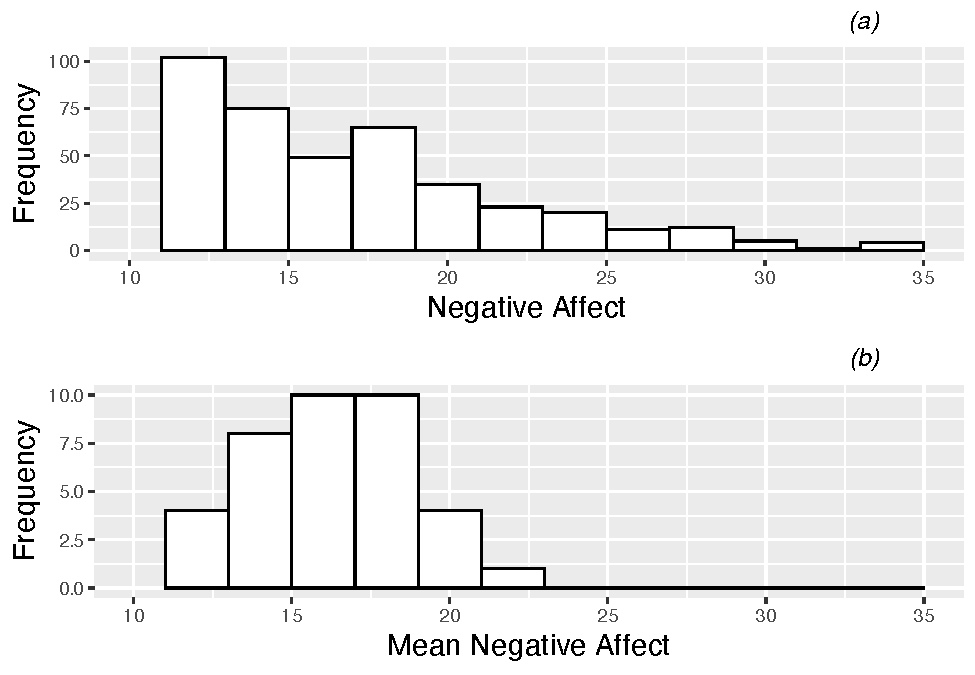
\includegraphics[width=0.6\linewidth]{bookdown-bysh_files/figure-latex/mli-hist1-1} 

}

\caption{Histogram of the continuous Level One response (negative effect). Plot (a) contains all 497 performances across the 37 musicians, while plot (b) contains one observation per musician (the mean negative affect across all performances).}\label{fig:mli-hist1}
\end{figure}

We can also summarize categorical Level One covariates across all (possibly correlated) observations to get a rough relative comparison of trends. 56.1\% of the 497 performances in our data set were solos, while 27.3\% were large ensembles and 16.5\% were small emsembles. The most common audience type was a public performance (41.0\%), followed by instructors (30.0\%), students (20.1\%), and finally juried recitals (8.9\%). In 30.0\% of performances, the musician played by memory, while 55.1\% used the score and 14.9\% of performances were unspecified.

To generate an initial examination of Level Two covariates, we consider a data set with just one observation per subject, since Level Two variables are constant over all performances from the same subject. Then, we can proceed as we did with Level One covariates---using histograms to illustrate the distributions of continuous covariates (see Figure \ref{fig:mli-histmat1}) and tables to summarize categorical covariates. For example, we learn that the majority of subjects have positive emotionality scores between 50 and 60, but that several subjects fall into a lengthy lower tail with scores between 20 and 50. A summary of categorical Level Two covariates reveals that among the 37 subjects (26 female and 11 male), 17 play an orchestral instrument, 15 are vocal performers, and 5 play a keyboard instrument.

\begin{figure}

{\centering 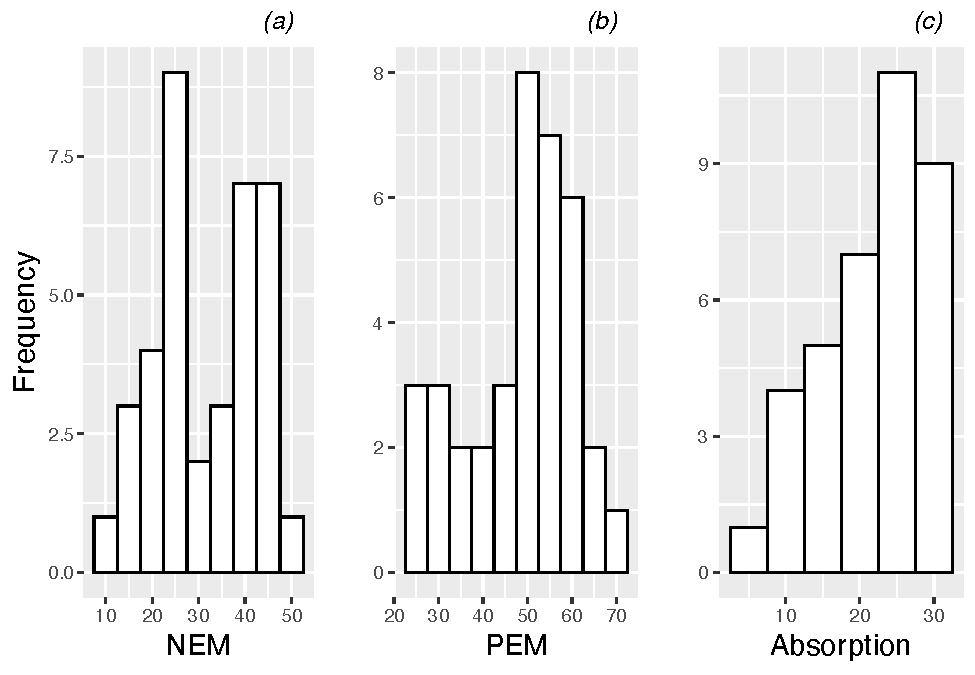
\includegraphics[width=0.6\linewidth]{bookdown-bysh_files/figure-latex/mli-histmat1-1} 

}

\caption{Histograms of the 3 continuous Level Two covariates (negative emotionality (NEM), positive emotionality (PEM), and absorption).  Each plot contains one observation per musician.}\label{fig:mli-histmat1}
\end{figure}

\hypertarget{explore2}{%
\subsection{Exploratory Analyses: Bivariate Summaries}\label{explore2}}

The next step in an initial exploratory analysis is the examination of numerical and graphical summaries of relationships between model covariates and responses. In examining these bivariate relationships, we hope to learn: (1) if there is a general trend suggesting that as the covariate increases the response either increases or decreases, (2) if subjects at certain levels of the covariate tend to have similar mean responses (low variability), and (3) if the variation in the response differs at different levels of the covariate (unequal variability).

As with individual variables, we will begin by treating all 497 performances recorded as independent observations, even though blocks of 15 or so performances were performed by the same musician. For categorical Level One covariates, we can generate boxplots against negative affect as in Figure \ref{fig:mli-boxscatmat1}, plots (a) and (b). From these boxplots, we see that lower levels of performance anxiety seem to be associated with playing in large ensembles and playing in front of an instructor. For our lone continuous Level One covariate (number of previous performances), we can generate a scatterplot against negative affect as in plot (c) from Figure \ref{fig:mli-boxscatmat1}, adding a fitted line to illustrate general trends upward or downward. From this scatterplot, we see that negative affect seems to decrease slightly as a subject has more experience.

To avoid the issue of dependent observations in our three plots from Figure \ref{fig:mli-boxscatmat1}, we could generate separate plots for each subject and examine trends within and across subjects. These ``lattice plots'' are illustrated in Figures \ref{fig:mli-lattice1}, \ref{fig:mli-lattice2}, and \ref{fig:mli-lattice3}; we discuss such plots more thoroughly in Chapter \ref{ch-lon}. While general trends are difficult to discern from these lattice plots, we can see the variety in subjects in sample size distributions and overall level of performance anxiety. In particular, in Figure \ref{fig:mli-lattice3}, we notice that linear fits for many subjects illustrate the same same slight downward trend displayed in the overall scatterplot in Figure \ref{fig:mli-boxscatmat1}, although some subjects experience increasing anxiety and others exhibit non-linear trends. Having an idea of the range of individual trends will be important when we begin to draw overall conclusions from this study.

\begin{figure}

{\centering 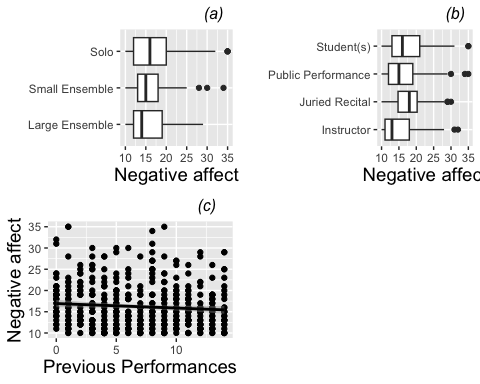
\includegraphics[width=0.6\linewidth]{bookdown-bysh_files/figure-latex/mli-boxscatmat1-1} 

}

\caption{Boxplots of two categorical Level One covariates (performance type (a) and audience type (b)) vs. model response, and scatterplot of one continuous Level One covariate (number of previous diary entries (c)) vs. model response (negative affect).  Each plot contains one observation for each of the 497 performances.}\label{fig:mli-boxscatmat1}
\end{figure}

\begin{figure}

{\centering 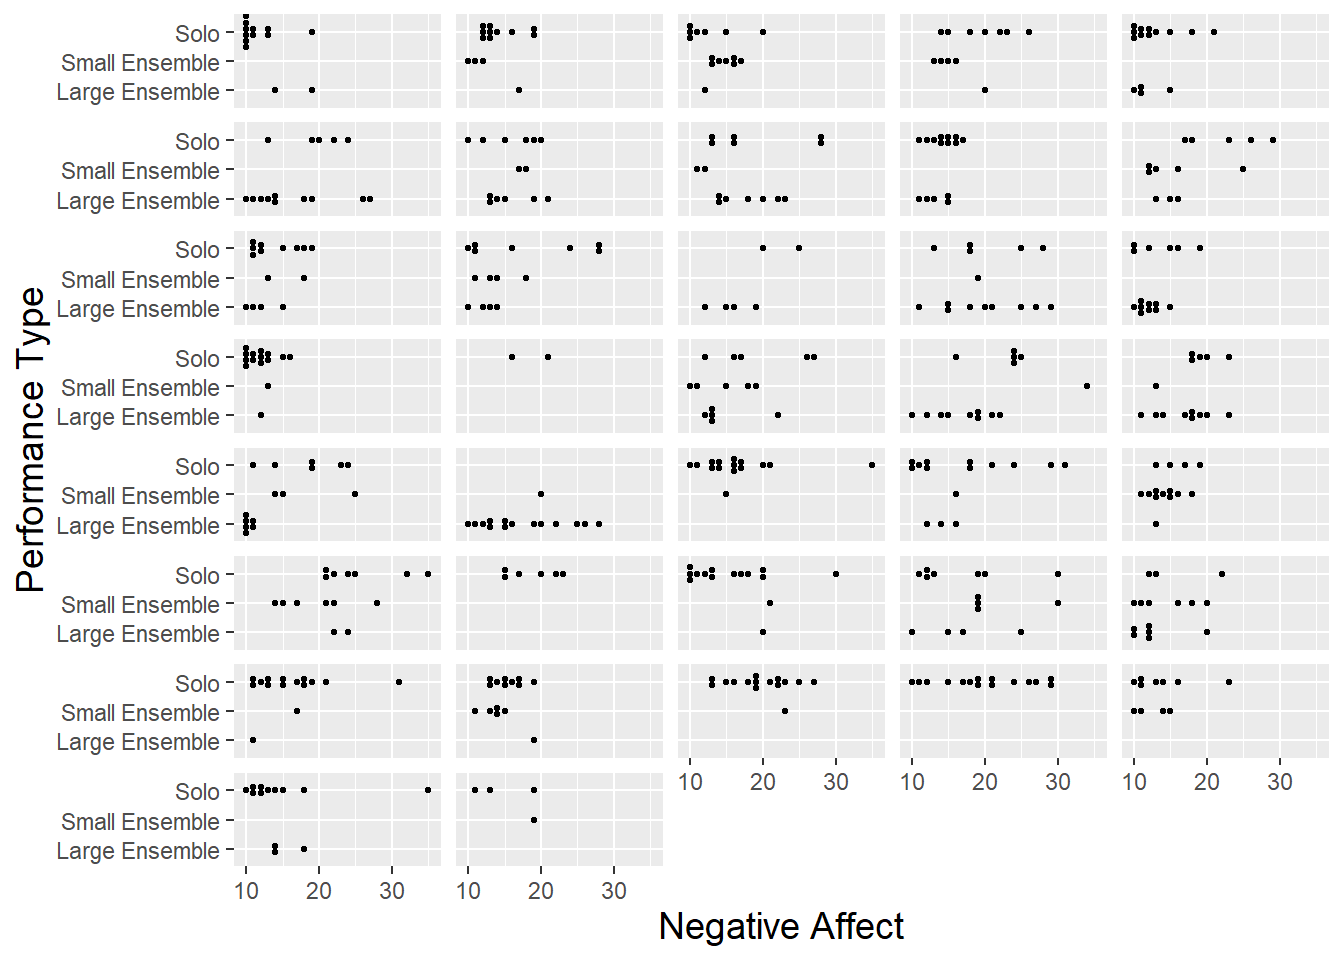
\includegraphics[width=0.6\linewidth]{bookdown-bysh_files/figure-latex/mli-lattice1-1} 

}

\caption{Lattice plot of performance type vs. negative affect, with separate dotplots by subject.}\label{fig:mli-lattice1}
\end{figure}

\begin{figure}

{\centering 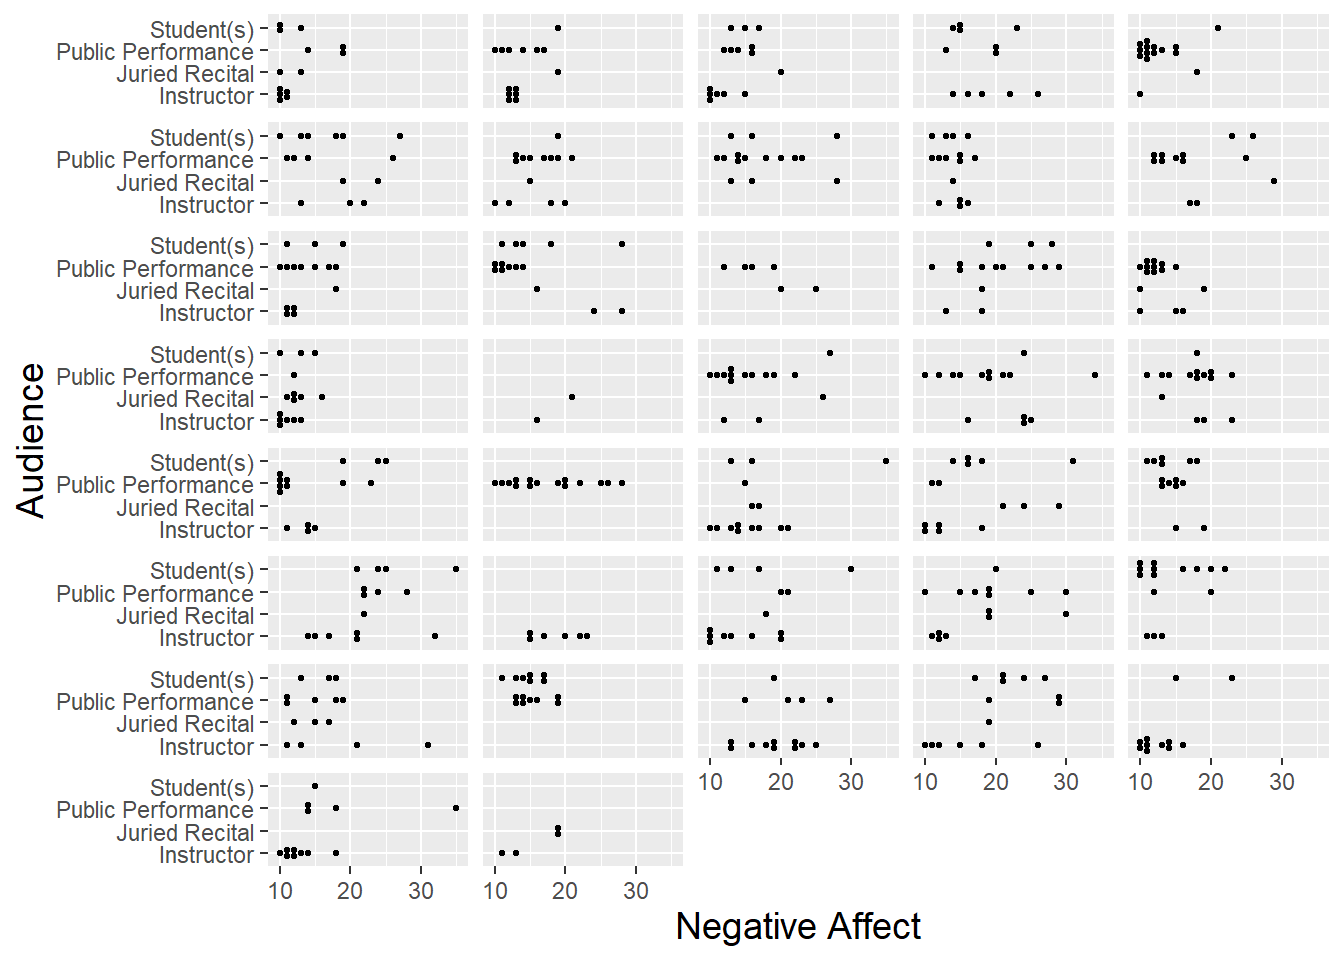
\includegraphics[width=0.6\linewidth]{bookdown-bysh_files/figure-latex/mli-lattice2-1} 

}

\caption{Lattice plot of audience type vs. negative affect, with separate dotplots by subject.}\label{fig:mli-lattice2}
\end{figure}

\begin{figure}

{\centering 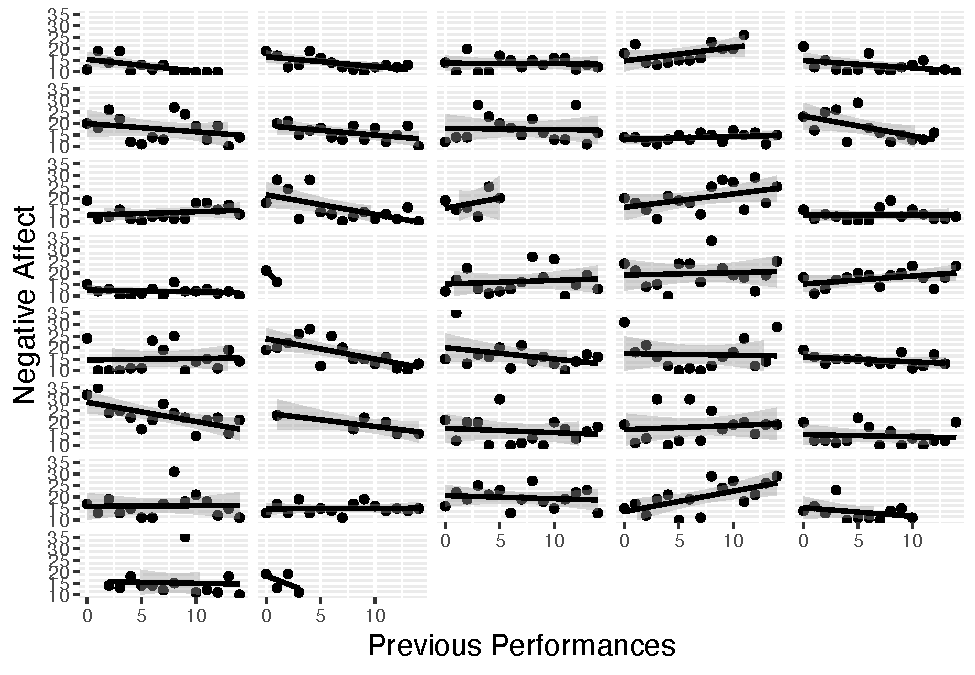
\includegraphics[width=0.6\linewidth]{bookdown-bysh_files/figure-latex/mli-lattice3-1} 

}

\caption{Lattice plot of previous performances vs. negative affect, with separate scatterplots with fitted lines by subject.}\label{fig:mli-lattice3}
\end{figure}

In Figure \ref{fig:mli-boxmat1}, we use boxplots to examine the relationship between our primary categorical Level Two covariate (instrument) and our continuous model response. Plot (a) uses all 497 performances, while plot (b) uses one observation per subject (the mean performance anxiety across all performances) regardless of how many performances that subject had. Naturally, plot (b) has a more condensed range of values, but both plots seem to support the notion that performance anxiety is slightly lower for vocalists and maybe a bit higher for keyboardists

\begin{figure}

{\centering 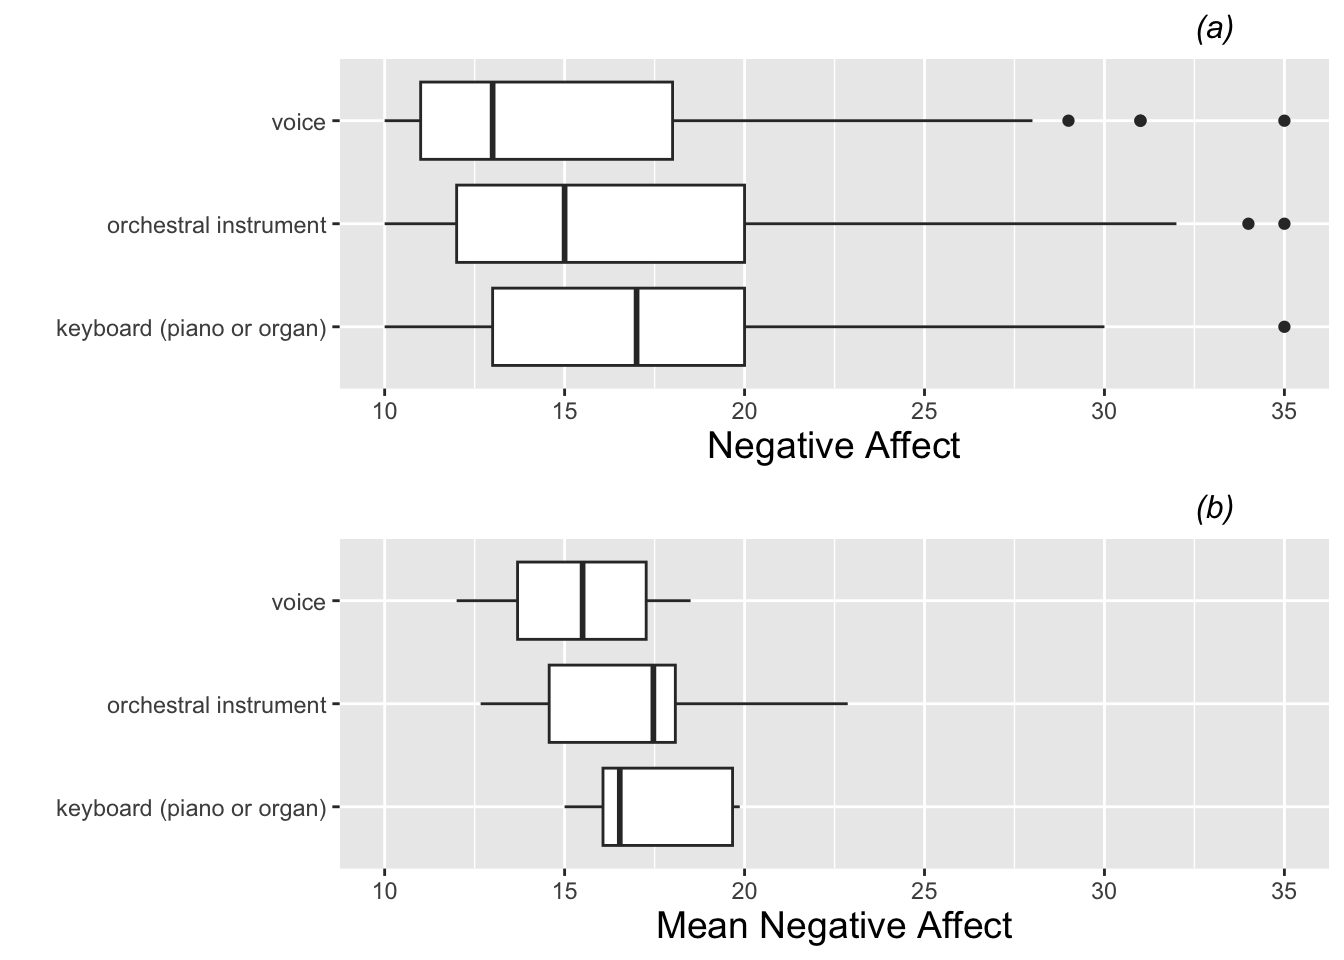
\includegraphics[width=0.6\linewidth]{bookdown-bysh_files/figure-latex/mli-boxmat1-1} 

}

\caption{Boxplots of the categorical Level Two covariate (instrument) vs. model response (negative affect).  Plot (a) is based on all 497 observations from all 37 subjects, while plot (b) uses only one observation per subject.}\label{fig:mli-boxmat1}
\end{figure}

In Figure \ref{fig:mli-scatmat1}, we use scatterplots to examine the relationships between continuous Level Two covariates and our model response. Performance anxiety appears to vary little with a subject's positive emotionality, but there is some evidence to suggest that performance anxiety increases with increasing negative emotionality and absorption level. Plots based on mean negative affect, with one observation per subject, support conclusions based on plots with all observations from all subjects; indeed the overall relationships are in the same direction and of the same magnitude.

\begin{figure}

{\centering 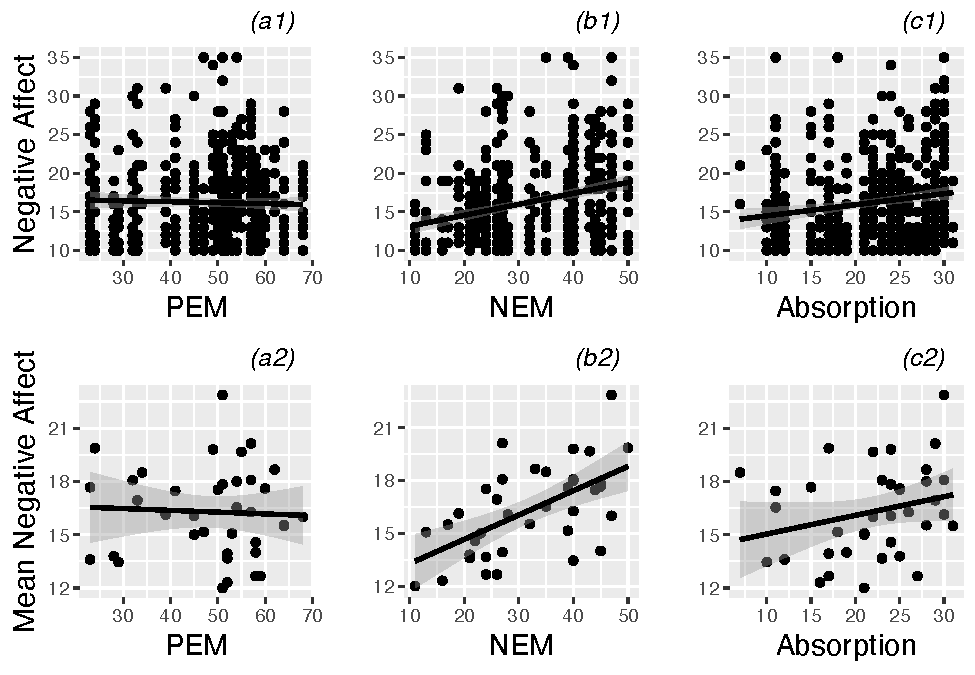
\includegraphics[width=0.6\linewidth]{bookdown-bysh_files/figure-latex/mli-scatmat1-1} 

}

\caption{ Scatterplots of continuous Level Two covariates (positive emotionality (PEM), negative emotionality (NEM), and absorption) vs. model response (negative affect).  The top plots (a1, b1, c1) are based on all 497 observations from all 37 subjects, while the bottom plots (a2, b2, c2) use only one observation per subject.}\label{fig:mli-scatmat1}
\end{figure}

Of course, any graphical analysis is exploratory, and any notable trends at this stage should be checked through formal modeling. At this point, a statistician begins to ask familiar questions such as:

\begin{itemize}
\tightlist
\item
  which characteristics of individual performances are most associated with performance anxiety?
\item
  which characteristics of study participants are most associated with performance anxiety?
\item
  are any of these associations statistically significant?
\item
  does the significance remain after controlling for other covariates?
\item
  how do we account for the lack of independence in performances by the same musician?
\end{itemize}

As you might expect, answers to these questions will arise from proper consideration of variability and properly identified statistical models.

\hypertarget{twolevelmodeling}{%
\section{Two level modeling: preliminary considerations}\label{twolevelmodeling}}

\hypertarget{multregr}{%
\subsection{Ignoring the two level structure (not recommended)}\label{multregr}}

Armed with any statistical software package, it would be relatively simple to take our complete data set of 497 observations and run an OLS multiple linear regression model seeking to explain variability in negative affect with a number of performance-level or musician-level covariates. As an example, output from a model with two binary covariates (Does the subject play an orchestral instrument? and, Was the performance a large ensemble?) is presented below. Do you see any problems with this approach?

\begin{verbatim}
lm(formula = na ~ orch + large + orch:large, data = music)

Coefficients:
            Estimate Std. Error t value Pr(>|t|)    
(Intercept)  15.7212     0.3591  43.778  < 2e-16 ***
orch          1.7887     0.5516   3.243  0.00126 ** 
large        -0.2767     0.7910  -0.350  0.72662    
orch:large   -1.7087     1.0621  -1.609  0.10831    
---
Residual standard error: 5.179 on 493 degrees of freedom
Multiple R-squared:  0.02782,   Adjusted R-squared:  0.0219 
F-statistic: 4.702 on 3 and 493 DF,  p-value: 0.003012
\end{verbatim}

Other than somewhat skewed residuals, residual plots (not shown) do not indicate any major problems with the OLS multiple regression model. However, another key assumption in these models is the independence of all observations. While we might reasonably conclude that responses from different study participants are independent (although possibly not if they are members of the same ensemble group), it is not likely that the 15 or so observations taken over multiple performances from a single subject are similarly independent. If a subject begins with a relatively high level of anxiety (compared to other subjects) before her first performance, chances are good that she will have relatively high anxiety levels before subsequent performances. Thus, OLS multiple linear regression using all 497 observations is not advisable for this study (or multilevel data sets in general).

\hypertarget{twostage}{%
\subsection{A two-stage modeling approach (better but imperfect)}\label{twostage}}

If we assume that the 37 study participants can reasonably be considered to be independent, we could use traditional OLS regression techniques to analyze data from this study if we could condense each subject's set of responses to a single meaningful outcome. Candidates for this meaningful outcome include a subject's last performance anxiety measurement, average performance anxiety, minimum anxiety level, etc. For example, in clinical trials, data is often collected over many weekly or monthly visits for each patient, except that many patients will drop out early for many reasons (e.g., lack of efficacy, side effects, personal reasons). In these cases, treatments are frequently compared using ``last-value-carried-forward'' methods---the final visit of each patient is used as the primary outcome measure, regardless of how long they remained in the study. However, ``last-value-carried-forward'' and other summary measures feel inadequate, since we end up ignoring much of the information contained in the multiple measures for each individual. A more powerful solution is to model performance anxiety at multiple levels.

We will begin by considering all performances by a single individual. For instance, consider the 15 performances for which Musician \#22 recorded a diary, illustrated in Table \ref{tab:table2chp8}.

\begin{table}

\caption{\label{tab:table2chp8}Data from the 15 performances of Musician 22}
\centering
\begin{tabular}[t]{lrrllrl}
\toprule
  & id & diary & perform\_type & audience & na & instrument\\
\midrule
240 & 22 & 1 & Solo & Instructor & 24 & orchestral instrument\\
241 & 22 & 2 & Large Ensemble & Public Performance & 21 & orchestral instrument\\
242 & 22 & 3 & Large Ensemble & Public Performance & 14 & orchestral instrument\\
243 & 22 & 4 & Large Ensemble & Public Performance & 15 & orchestral instrument\\
244 & 22 & 5 & Large Ensemble & Public Performance & 10 & orchestral instrument\\
\addlinespace
245 & 22 & 6 & Solo & Instructor & 24 & orchestral instrument\\
246 & 22 & 7 & Solo & Student(s) & 24 & orchestral instrument\\
247 & 22 & 8 & Solo & Instructor & 16 & orchestral instrument\\
248 & 22 & 9 & Small Ensemble & Public Performance & 34 & orchestral instrument\\
249 & 22 & 10 & Large Ensemble & Public Performance & 22 & orchestral instrument\\
\addlinespace
250 & 22 & 11 & Large Ensemble & Public Performance & 19 & orchestral instrument\\
251 & 22 & 12 & Large Ensemble & Public Performance & 18 & orchestral instrument\\
252 & 22 & 13 & Large Ensemble & Public Performance & 12 & orchestral instrument\\
253 & 22 & 14 & Large Ensemble & Public Performance & 19 & orchestral instrument\\
254 & 22 & 15 & Solo & Instructor & 25 & orchestral instrument\\
\bottomrule
\end{tabular}
\end{table}

Does this musician tend to have higher anxiety levels when he is playing in a large ensemble or playing in front of fellow students? Which factor is the biggest determinant of anxiety for a performance by Musician \#22? We can address these questions through OLS multiple linear regression applied to only Musician \#22's data, using appropriate indicator variables for factors of interest.

Let \(Y_{j}\) be the performance anxiety score of Musician \#22 before performance \(j\). Consider the observed performances for Musician \#22 to be a random sample of all conceivable performances by that subject. If we are initially interested in examining the effect of playing in a large ensemble, we can model the performance anxiety for Musician \#22 according to the model:
\begin{equation}
Y_{22j}=a_{22}+b_{22}\textstyle{LargeEns}_{22j}+\epsilon_{22j} \textrm{ where } \epsilon_{22j}\sim N(0,\sigma^2) \textrm{ and }
\label{eq:level1a}
\end{equation}
\[ \textstyle{LargeEns}_{j} = \left\{ \begin{array}{ll}
                                1 & \textrm{if perf_type = Large Ensemble}\\
                                0 & \textrm{if perf_type = Solo or Small Ensemble.}
                                        \end{array}
                                \right.  \]
The parameters in this model (\(a_{22}\), \(b_{22}\), and \(\sigma^2\)) can be estimated through OLS methods. \(a_{22}\) represents the true intercept for Musician \#22---the expected anxiety score for Musician \#22 when performance type is a Solo or Small Ensemble (\(\textstyle{LargeEns}=0\)), or the true average anxiety for Musician \#22 over all Solo or Small Ensemble performances he may conceivably give. \(b_{22}\) represents the true slope for Musician \#22---the expected increase in performance anxiety for Musician \#22 when performing as part of a Large Ensemble rather than in a Small Ensemble or as a Solo, or the true average difference in anxiety scores for Musician \#22 between Large Ensemble performances and other types. Finally, the \(\epsilon_{22j}\) terms represent the deviations of Musician \#22's actual performance anxiety scores from the expected scores under this model---the part of Musician \#22's anxiety before performance \(j\) that is not explained by performance type. The variability in these deviations from the regression model is denoted by \(\sigma^2\).

For Subject 22, we estimate \(\hat{a}_{22}=24.5\), \(\hat{b}_{22}=-7.8\), and \(\hat{\sigma}=4.8\). Thus, according to our simple linear regression model, Subject 22 had an estimated anxiety score of 24.5 before Solo and Small Ensemble performances, and 16.7 (7.8 points lower) before Large Ensemble performances. With an \(R^2\) of 0.425, the regression model explains a moderate amount (42.5\%) of the performance-to-performance variability in anxiety scores for Subject 22, and the trend toward lower scores for large ensemble performances is statistically significant at the 0.05 level (t(13)=-3.10, p=.009).

\begin{verbatim}
lm(formula = na ~ large, data = id22)

Coefficients:
            Estimate Std. Error t value Pr(>|t|)    
(Intercept)   24.500      1.960  12.503 1.28e-08 ***
large         -7.833      2.530  -3.097   0.0085 ** 
---
Residual standard error: 4.8 on 13 degrees of freedom
Multiple R-squared:  0.4245,    Adjusted R-squared:  0.3802 
F-statistic: 9.588 on 1 and 13 DF,  p-value: 0.008504
\end{verbatim}

We could continue trying to build a better model for Subject 22, adding indicators for audience and memory, and even adding a continuous variable representing the number of previous performance where a diary was kept. As our model R-square value increased, we would be explaining a larger proportion of Subject 22's performance-to-performance variability in anxiety. It would not, however, improve our model to incorporate predictors for age, gender, or even negative emotionality based on the MPQ---why is that?

For the present time, we will model Subject 22's anxiety scores for his 15 performances using the model given by Equation \eqref{eq:level1a}, with a lone indicator variable for performing in a Large Ensemble. We can then proceed to fit the OLS regression model in Equation \eqref{eq:level1a} to examine the effect of performing in a Large Ensemble for each of the 37 subjects in this study. These are called \textbf{Level One models}. As displayed in Figure \ref{fig:mli-histmat2}, there is considerable variability in the fitted intercepts and slopes among the 37 subjects. Mean performance anxiety scores for Solos and Small Ensembles range from 11.6 to 24.5, with a median score of 16.7, while mean differences in performance anxiety scores for Large Ensembles compared to Solos and Small Ensembles range from -7.9 to 5.0, with a median difference of -1.7. Can these differences among individual musicians be explained by (performance-invariant) characteristics associated with each individual, such as gender, age, instrument, years studied, or baseline levels of personality measures? Questions like these can be addressed through further statistical modeling.

\begin{figure}

{\centering 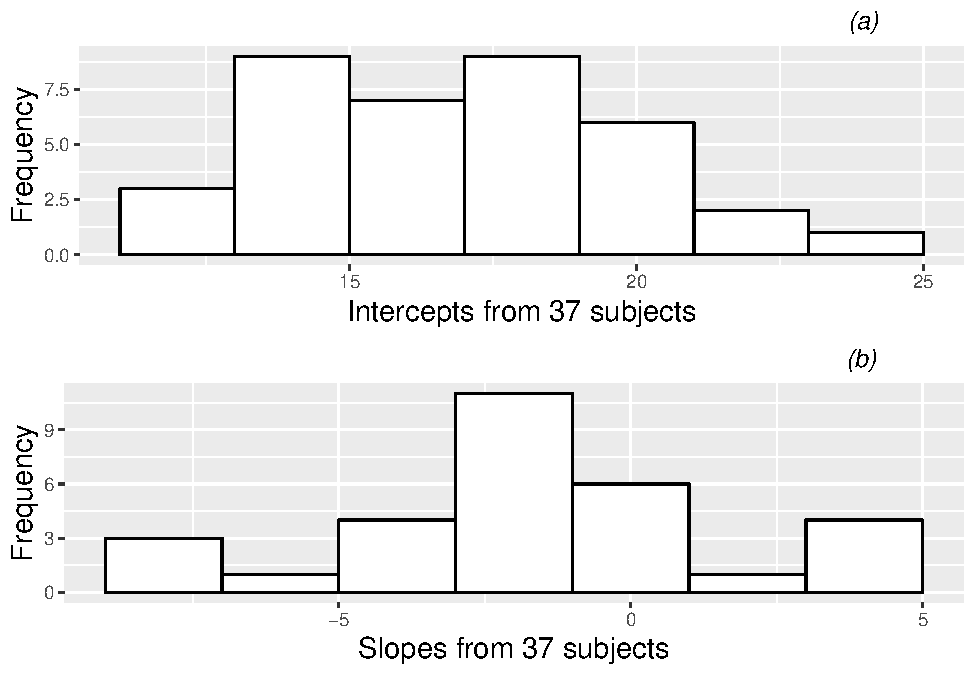
\includegraphics[width=0.6\linewidth]{bookdown-bysh_files/figure-latex/mli-histmat2-1} 

}

\caption{Histograms of intercepts and slopes from fitting simple regression models by subject, where each model contained a single binary predictor indicating if a performance was part of a large ensemble.}\label{fig:mli-histmat2}
\end{figure}

As an illustration, we can consider whether or not there are significant relationships between individual regression parameters (intercepts and slopes) and instrument played. From a modeling perspective, we would build a system of two \textbf{Level Two models} to predict the fitted intercept (\(a_{i}\)) and fitted slopes (\(b_{i}\)) for Subject \(i\):
\begin{eqnarray}
a_{i} & = & \alpha_{0}+\alpha_{1}\textstyle{Orch}_{i}+u_{i}
\label{eq:level2s0}  \\
b_{i} & = & \beta_{0}+\beta_{1}\textstyle{Orch}_{i}+v_{i}
\label{eq:level2s1}
\end{eqnarray}
where \(\textstyle{Orch}_{i}=1\) if Subject \(i\) plays an orchestral instrument and \(\textstyle{Orch}_{i}=0\) if Subject \(i\) plays keyboard or is a vocalist. Note that, at Level Two, our response variables are not observed measurements such as performance anxiety scores, but rather the fitted regression coefficients from the Level One models fit to each subject. (Well, in our theoretical model, the responses are actually the true intercepts and slopes from Level One models for each subject, but in reality, we have to use our estimated slopes and intercepts.)

Exploratory data analysis (see boxplots by instrument in Figure \ref{fig:mli-boxmat2} suggests that subjects playing orchestral instruments have higher intercepts than vocalists or keyboardists, and that orchestral instruments are associated with slight lower (more negative) slopes, although with less variability that the slopes of vocalists and keyboardists. These trends are borne out in regression modeling. If we fit Equations \eqref{eq:level2s0} and \eqref{eq:level2s1} using fitted intercepts and slopes as our response variables, we obtain the following estimated parameters: \(\hat{\alpha}_{0}=16.3\), \(\hat{\alpha}_{1}=1.4\), \(\hat{\beta}_{0}=-0.8\), and \(\hat{\beta}_{1}=-1.4\). Thus, the intercept (\(a_{i}\)) and slope (\(b_{i}\)) for Subject \(i\) can be modeled as:
\begin{eqnarray}
\hat{a}_{i} & = & 16.3+1.4\textstyle{Orch}_{i}+u_{i}
\label{eq:level2s0hat}  \\
\hat{b}_{i} & = & -0.8-1.4\textstyle{Orch}_{i}+v_{i}
\label{eq:level2s1hat}
\end{eqnarray}

where \(a_{i}\) is the true mean negative affect when Subject \(i\) is playing solos or small ensembles, and \(b_{i}\) is the true mean difference in negative affect for Subject \(i\) between large ensembles and other performance types. Based on these models, average performance anxiety before solos and small ensembles is 16.3 for vocalists and keyboardists, but 17.7 (1.4 points higher) for orchestral instrumentalists. Before playing in large ensembles, vocalists and instrumentalists have performance anxiety (15.5) which is 0.8 points lower, on average, than before solos and small ensembles, while subjects playing orchestral instruments experience an average difference of 2.2 points, producing an average performance anxiety of 15.5 before playing in large ensembles just like subjects playing other instruments. However, the difference between orchestral instruments and others does not appear to be statistically significant for either intercepts (t=1.424, p=0.163) or slopes (t=-1.168, p=0.253).

\begin{figure}

{\centering 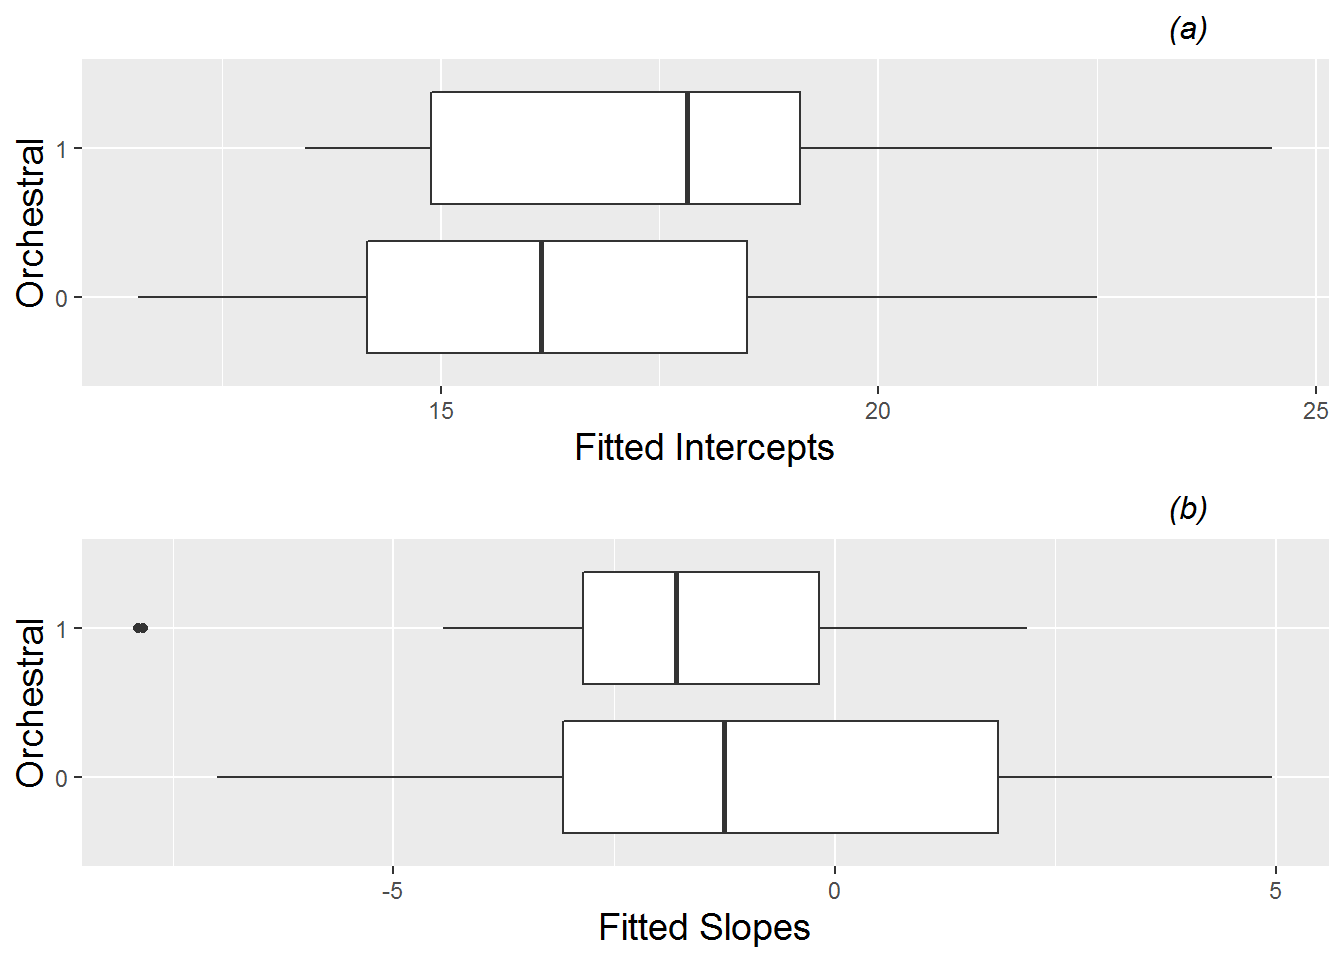
\includegraphics[width=0.6\linewidth]{bookdown-bysh_files/figure-latex/mli-boxmat2-1} 

}

\caption{Boxplots of fitted intercepts (plot (a)) and slopes (plot (b)) by orchestral instrument (1) vs. keyboard or vocalist (0).}\label{fig:mli-boxmat2}
\end{figure}

This two stage modeling process does have some drawbacks. Among other things, (1) it weights every subject the same regardless of the number of diary entries we have, (2) it responds to missing individual slopes (from 7 subjects who never performed in a large ensemble) by simply dropping those subjects, and (3) it does not share strength effectively across individuals. These issues can be better handled through a unified multilevel modeling framework which we will develop over the remainder of this section.

\hypertarget{twolevelmodelingunified}{%
\section{Two level modeling: a unified approach}\label{twolevelmodelingunified}}

\hypertarget{ourframework}{%
\subsection{Our framework}\label{ourframework}}

For the unified approach, we will still envision two levels of models as in section \ref{twostage}, but we will use likelihood-based methods for parameter estimation rather than ordinary least squares to address the drawbacks associated with the two-stage approach. To illustrate the unified approach, we will first generalize the models presented in section \ref{twostage}. Let \(Y_{ij}\) be the performance anxiety score of the \(i^{th}\) subject before performance \(j\). If we are initially interested in examining the effects of playing in a large ensemble and playing an orchestral instrument, then we can model the performance anxiety for Subject \(i\) in performance \(j\) with the following system of equations:

\begin{itemize}
\tightlist
\item
  Level One:
  \begin{equation}
  Y_{ij} = a_{i}+b_{i}\textstyle{LargeEns}_{ij}+\epsilon_{ij}
  \label{eq:level1large}
  \end{equation}
\item
  Level Two:
  \begin{eqnarray*}
  a_{i} & = & \alpha_{0}+\alpha_{1}\textstyle{Orch}_{i}+u_{i} \\
  b_{i} & = & \beta_{0}+\beta_{1}\textstyle{Orch}_{i}+v_{i},
  \end{eqnarray*}
\end{itemize}

In this system, there are 4 key \textbf{fixed effects} to estimate: \(\alpha_{0}\), \(\alpha_{1}\), \(\beta_{0}\) and \(\beta_{1}\). Fixed effects are the fixed but unknown population effects associated with certain covariates. The intercepts and slopes for each subject from Level One, \(a_{i}\) and \(b_{i}\), don't need to be formally estimated as we did in section \ref{twostage}; they serve to conceptually connect Level One with Level Two. In fact, by substituting the two Level Two equations into the Level One equation, we can view this two-level system of models as a single \textbf{Composite Model} without \(a_{i}\) and \(b_{i}\):
\begin{eqnarray*}
Y_{ij} & = & [\alpha_{0}+\alpha_{1}\textstyle{Orch}_{i}+\beta_{0}\textstyle{LargeEns}_{ij}+\beta_{1}\textstyle{Orch}_{i}\textstyle{LargeEns}_{ij}] \\
 & & \textrm{} + [u_{i}+v_{i}\textstyle{LargeEns}_{ij}+\epsilon_{ij}]
\end{eqnarray*}

From this point forward, when building multilevel models, we will use Greek letters (such as \(\alpha_{0}\)) to denote final fixed effects model parameters to be estimated empirically, and Roman letters (such as \(a_{0}\)) to denote preliminary fixed effects parameters at lower levels. Variance components that will be estimated empirically will be denoted with \(\sigma\) or \(\rho\), while terms such as \(\epsilon\) and \(u_{i}\) represent error terms. In our framework, we can estimate final parameters directly without first estimating preliminary parameters, which can be seen with the Composite Model formulation (although we can obtain estimates of preliminary parameters in those occasional cases when they are of interest to us). Note that when we model a slope term like \(b_{i}\) from Level One using Level Two covariates like \(\textstyle{Orch}_{i}\), the resulting Composite Model contains an \textbf{interaction term}, denoting that the effect of \(\textstyle{LargeEns}_{ij}\) depends on the instrument played.

Furthermore, with a binary predictor at Level Two such as instrument, we can write out what our Level Two model looks like for those who play keyboard or are vocalists (\(\textstyle{Orch}_{i}=0\)) and those who play orchestral instruments (\(\textstyle{Orch}_{i}=1\)):

\begin{itemize}
\tightlist
\item
  Keyboardists and Vocalists (\(\textstyle{Orch}_{i}=0\))
  \begin{eqnarray*}
  a_{i} & = & \alpha_{0}+u_{i} \\
  b_{i} & = & \beta_{0}+v_{i}
  \end{eqnarray*}
\item
  Orchestral instrumentalists (\(\textstyle{Orch}_{i}=1\))
  \begin{eqnarray*}
  a_{i} & = & (\alpha_{0}+\alpha_{1})+u_{i} \\
  b_{i} & = & (\beta_{0}+\beta_{1})+v_{i}
  \label{eq:level2byorch}
  \end{eqnarray*}
\end{itemize}

Writing the Level Two model in this manner helps us interpret the model parameters from our two-level model. In this case, even the Level One covariate is binary, so that we can write out expressions for mean performance anxiety based on our model for four different combinations of instrument played and performance type:

\begin{itemize}
\tightlist
\item
  Keyboardists or vocalists playing solos or small ensembles: \(\alpha_{0}\)
\item
  Keyboardists or vocalists playing large ensembles: \(\alpha_{0}+\beta_{0}\)
\item
  Orchestral instrumentalists playing solos or small ensembles: \(\alpha_{0}+\alpha_{1}\)
\item
  Orchestral instrumentalists playing large ensembles: \(\alpha_{0}+\alpha_{1}+\beta_{0}+\beta_{1}\)
\end{itemize}

\hypertarget{random-vs.-fixed-effects}{%
\subsection{Random vs.~fixed effects}\label{random-vs.-fixed-effects}}

Before we can use likelihood-based methods to estimate our model parameters, we still must define the distributions of our error terms. The error terms \(\epsilon_{ij}\), \(u_{i}\), and \(v_{i}\) represent random effects in our model. In multilevel models, it is important to distinguish between fixed and random effects. Typically, \textbf{fixed effects} describe levels of a factor that we are specifically interested in drawing inferences about, and which would not change in replications of the study. For example, in our music performance anxiety case study, the levels of performance type will most likely remain as solos, small ensembles, and large ensembles even in replications of the study, and we wish to draw specific conclusions about differences between these three types of performances. Thus, performance type would be considered a fixed effect. On the other hand, \textbf{random effects} describe levels of a factor which can be thought of as a sample from a larger population of factor levels; we are not typically interested in drawing conclusions about specific levels of a random effect, although we are interested in accounting for the influence of the random effect in our model. For example, in our case study the different musicians included can be thought of as a random sample from a population of performing musicians. Although our goal is not to make specific conclusions about differences between any two musicians, we do want to account for inherent differences among musicians in our model, and by doing so, we will be able to draw more precise conclusions about our fixed effects of interest. Thus, musician would be considered a random effect.

\hypertarget{MVN}{%
\subsection{Distribution of errors: the multivariate normal distribution}\label{MVN}}

As part of our multilevel model, we must provide probability distributions to describe the behavior of random effects. Typically, we assume that random effects follow a normal distribution with mean 0 and a variance parameter which must be estimated from the data. For example, at Level One, we will assume that the errors associated with each performance of a particular musician can be described as: \(\epsilon_{ij}\sim N(0,\sigma^2)\). At Level Two, we have one error term (\(u_{i}\)) associated with subject-to-subject differences in intercepts, and one error term (\(v_{i}\)) associated with subject-to-subject differences in slopes. That is, \(u_{i}\) represents the deviation of Subject \(i\) from the mean performance anxiety before solos and small ensembles after accounting for his or her instrument, and \(v_{i}\) represents the deviation of Subject \(i\) from the mean difference in performance anxiety between large ensembles and other performance types after accounting for his or her instrument.

In modeling the random behavior of \(u_{i}\) and \(v_{i}\), we must also account for the possibility that random effects at the same level might be correlated. Subjects with higher baseline performance anxiety have a greater capacity for showing decreased anxiety in large ensembles as compared to solos and small ensembles, so we might expect that subjects with larger intercepts (performance anxiety before solos and small ensembles) would have smaller slopes (indicating greater decreases in anxiety before large ensembles). In fact, our fitted Level One intercepts and slopes in this example actually show evidence of a fairly strong negative correlation (\(r=-0.525\), see Figure \ref{fig:mli-scat1}).

\begin{figure}

{\centering 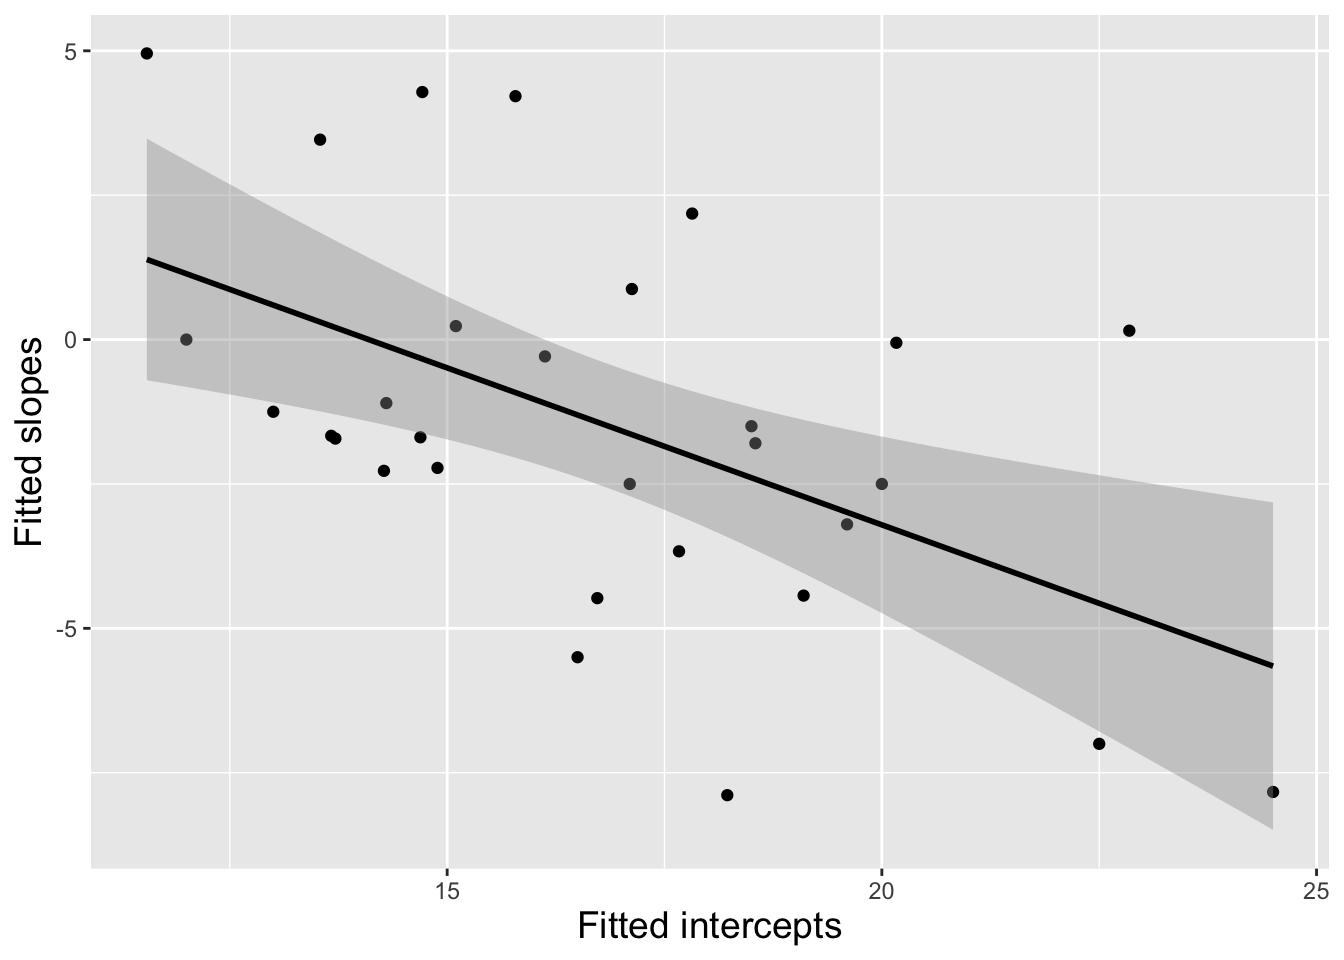
\includegraphics[width=0.6\linewidth]{bookdown-bysh_files/figure-latex/mli-scat1-1} 

}

\caption{Scatterplot with fitted regression line for estimated intercepts and slopes (one point per subject).}\label{fig:mli-scat1}
\end{figure}

To allow for this correlation, the error terms at Level Two can be assumed to follow a multivariate normal distribution in our unified multilevel model. Mathematically, we can express this as:
\[ \left[ \begin{array}{c}
            u_{i} \\ v_{i}
          \end{array}  \right] \sim N \left( \left[
          \begin{array}{c}
            0 \\ 0
          \end{array} \right], \left[
          \begin{array}{cc}
            \sigma_{u}^{2} & \\
            \rho_{uv}\sigma_{u}\sigma_v & \sigma_{v}^{2}
          \end{array} \right] \right) \]
Note that the correlation \(\rho_{uv}\) between the error terms is simply the covariance \(\sigma_{uv}=\rho_{uv}\sigma_{u}\sigma_{v}\) converted to a \([-1,1]\) scale through the relationship:
\begin{equation}
\rho_{uv} = \frac{\rho\sigma_{u}\sigma_{v}}{\sigma_{u}\sigma_{v}}
\label{eq:cor}
\end{equation}

With this expression, we are allowing each error term to have its own variance (around a mean of 0) and each pair of error terms to have its own covariance (or correlation). Thus, if there are \(n\) equations at Level Two, we can have \(n\) variance terms and \(n(n-1)/2\) covariance terms for a total of \(n + n(n-1)/2\) variance components. These variance components are organized in matrix form, with variance terms along the diagonal and covariance terms in the off-diagonal. In our small example, we have \(n=2\) equations at Level Two, so we have 3 variance components to estimate---2 variance terms (\(\sigma_{u}^{2}\) and \(\sigma_{v}^{2}\)) and 1 covariance term (\(\sigma_{uv}\)).

The multivariate normal distribution with \(n=2\) is illustrated in Figure \ref{fig:contour-boundary} for two cases: (a) the error terms are uncorrelated (\(\sigma_{uv}=\rho_{uv}=0\)), and (b) the error terms are positively correlated (\(\sigma_{uv}>0\) and \(\rho_{uv} > 0\)). In general, if the errors in intercepts (\(u_{i}\)) are placed on the x-axis and the errors in slopes (\(v_{i}\)) are placed on the y-axis, then \(\sigma_{u}^{2}\) measures spread in the x-direction and \(\sigma_{v}^{2}\) measures spread in the y-direction, while \(\sigma_{uv}\) measures tilt. Positive tilt (\(\sigma_{uv}>0\)) indicates a tendency for errors from the same subject to both be positive or both be negative, while negative tilt (\(\sigma_{uv}<0\)) indicates a tendency for one error from a subject to be positive and the other to be negative. In Figure \ref{fig:contour-boundary}, \(\sigma_{u}^{2}=4\) and \(\sigma_{v}^{2}=1\), so both contour plots show a greater range of errors in the x-direction than the y-direction. Internal ellipses in the contour plot indicate pairs of \(u_{i}\) and \(v_{i}\) that are more likely. In Figure \ref{fig:contour-boundary} (a) \(\sigma_{uv}=\rho_{uv}=0\), so the axes of the contour plot correspond to the x- and y-axes, but in Figure \ref{fig:contour-boundary} (b) \(\sigma_{uv}=1.5\), so the contour plot tilts up, reflecting a tendency for high values of \(u_{i}\) to be associated with high values of \(v_{i}\).

\begin{figure}

{\centering 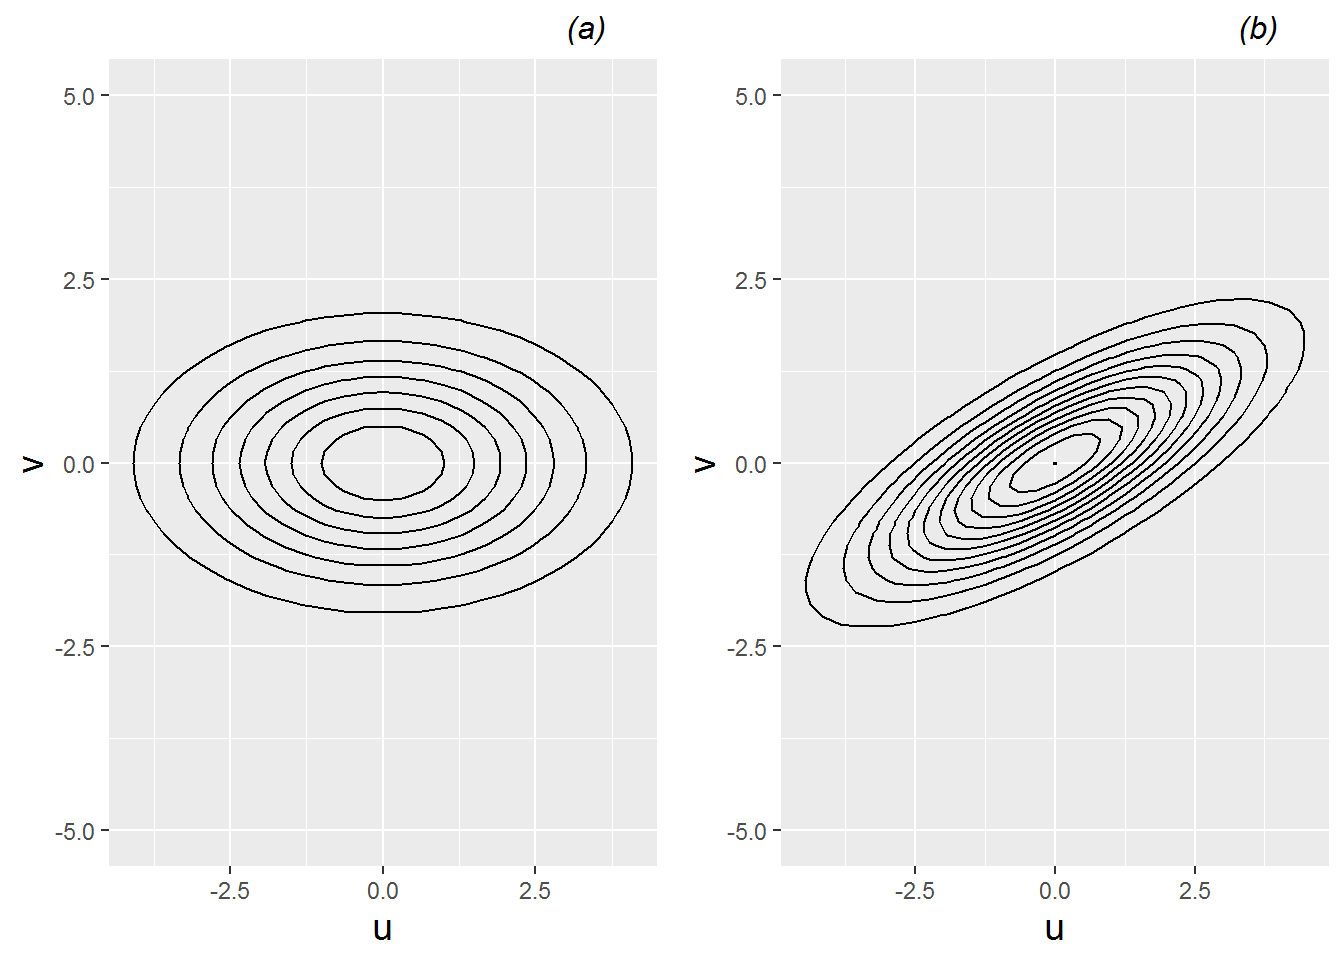
\includegraphics[width=0.6\linewidth]{bookdown-bysh_files/figure-latex/contour-boundary-1} 

}

\caption{Contour plots illustrating multivariate normal density with (a) no correlation between error terms, and (b) positive correlation between error terms.}\label{fig:contour-boundary}
\end{figure}

\hypertarget{multileveltechnical}{%
\subsection{Technical issues when estimating and testing parameters (Optional)}\label{multileveltechnical}}

Now, our two-level model has 8 parameters that need to be estimated: 4 fixed effects (\(\alpha_{0}\), \(\alpha_{1}\), \(\beta_{0}\), and \(\beta_{1}\)), and 4 variance components (\(\sigma^{2}\), \(\sigma_{u}^{2}\), \(\sigma_{v}^{2}\), and \(\sigma_{uv}\)). Note that we use the term \textbf{variance components} to signify model parameters that describe the behavior of random effects. We can use statistical software, such as the lmer() function from the lme4 package in R, to obtain parameter estimates using our 497 observations. The most common methods for estimating model parameters---both fixed effects and variance components---are maximum likelihood (ML) and restricted maximum likelihood (REML). The method of maximum likelihood (ML) was introduced in Chapter \ref{ch-beyondmost}, where parameter estimates are chosen to maximize the value of the likelihood function based on observed data. Restricted maximum likelihood (REML) is conditional on the fixed effects, so that the part of the data used for estimating variance components is separated from that used for estimating fixed effects. Thus REML, by accounting for the loss in degrees of freedom from estimating the fixed effects, provides an unbiased estimate of variance components, while ML estimators for variance components are biased under assumptions of normality, since they use estimated fixed effects rather than the true values. REML is preferable when the number of parameters is large or the primary interest is obtaining estimates of model parameters, either fixed effects or variance components associated with random effects. ML should be used if nested fixed effects models are being compared using a likelihood ratio test, although REML is fine for nested models of random effects (with the same fixed effects model). In this text, we will typically report REML estimates unless we are specifically comparing nested models with the same random effects. In most case studies and most models we consider, there is very little difference between ML and REML parameter estimates. Additional details are beyond the scope of this book \citep{Singer2003}.

Note that the multilevel output shown beginning in the next section contains no p-values for performing hypothesis tests. This is primarily because the exact distribution of the test statistics under the null hypothesis (no fixed effect) is unknown, primarily because the exact degrees of freedom is not known \citep{Bates2015}. Finding good approximate distributions for test statistics (and thus good approximate p-values) in multilevel models is an area of active research. In most cases, we can simply conclude that t-values (ratios of parameter estimates to estimated standard errors) with absolute value above 2 indicate significant evidence that a particular model parameter is different than 0. Certain software packages will report p-values corresponding to hypothesis tests for parameters of fixed effects; these packages are typically using conservative assumptions, large-sample results, or approximate degrees of freedom for a t-distribution. In section \ref{multreg-boot}, we introduced the bootstrap as a non-parametric, computational approach for producing confidence intervals for model parameters. In addition, in section \ref{threelevel-paraboot}, we will introduce a method called the parametric bootstrap which is being used more frequently by researchers to better approximate the distribution of the likelihood test statistic and produce more accurate p-values by simulating data under the null hypothesis \citep{Efron2012}.

\hypertarget{initialmodel}{%
\subsection{An initial model with parameter interpretations}\label{initialmodel}}

The output below contains likelihood-based estimates of our 8 parameters from a two-level model applied to the music performance anxiety data:

\begin{verbatim}
    Linear mixed model fit by REML ['lmerMod'] 
 A)  Formula: na ~ orch + large + orch:large + (large | id) 
        Data: music 
 B)  REML criterion at convergence: 2987 
      
 B2)      AIC      BIC   logLik deviance df.resid  
       3007.2   3040.9  -1495.6   2991.2      489  
      
     Random effects: 
      Groups   Name        Variance Std.Dev. Corr  
 C)   id       (Intercept)  5.6555  2.378          
 D)            large        0.4529  0.673    -0.63 
 E)   Residual             21.8073  4.670          
 F)  Number of obs: 497, groups:  id, 37 
      
     Fixed effects: 
                 Estimate Std. Error t value 
 G)  (Intercept)  15.9297     0.6415  24.833 
 H)  orch          1.6926     0.9452   1.791 
 I)  large        -0.9106     0.8453  -1.077 
 J)  orch:large   -1.4239     1.0993  -1.295
\end{verbatim}

This output (except for the capital letters along the left column) was specifically generated by the lmer() function in R; multilevel modeling results from other packages will contain similar elements. Because we will use lmer() output to summarize analyses of case studies in this and following sections, we will spend a little time now orienting ourselves to the most important features in this output.

\begin{itemize}
\tightlist
\item
  A: How our multilevel model is written in R, based on the composite model formulation. For more details, see section \ref{notesr8}.
\item
  B: Measures of model performance. Since this model was fit using REML, this line only contains the REML criterion.
\item
  B2: If the model is fit with ML instead of REML, the measures of performance will contain AIC, BIC, deviance, and the log-likelihood.
\item
  C: Estimated variance components (\(\hat{\sigma}_{u}^2\) and \(\hat{\sigma}_{u}\)) associated with the intercept equation in Level Two.
\item
  D: Estimated variance components (\(\hat{\sigma}_{v}^2\) and \(\hat{\sigma}_{v}\)) associated with the large ensemble effect equation in Level Two, along with the estimated correlation (\(\hat{\rho}_{uv}\)) between the two Level Two error terms.
\item
  E: Estimated variance components (\(\hat{\sigma}^2\) and \(\hat{\sigma}\)) associated with the Level One equation.
\item
  F: Total number of performances where data was collected (Level One observations = 497) and total number of subjects (Level Two observations = 37).
\item
  G: Estimated fixed effect (\(\hat{\alpha}_{0}\)) for intercept term, along with its standard error and t-value (which is the ratio of the estimated coefficient to its standard error). As described in section \ref{multileveltechnical}, no p-value testing the significance of the coefficient is provided because the exact null distribution of the t-value is unknown.
\item
  H: Estimated fixed effect (\(\hat{\alpha}_{1}\)) for the orchestral instrument effect, along with its standard error and t-value .
\item
  I: Estimated fixed effect (\(\hat{\beta}_{0}\)) for the large ensemble effect, along with its standard error and t-value.
\item
  J: Estimated fixed effect (\(\hat{\beta}_{1}\)) for the interaction between orchestral instruments and large ensembles, along with its standard error and t-value.
\end{itemize}

Assuming the 37 musicians in this study are representative of a larger population of musicians, parameter interpretations for our 8 model parameters are given below:

\begin{itemize}
\tightlist
\item
  Fixed effects:

  \begin{itemize}
  \tightlist
  \item
    \(\hat{\alpha}_{0} = 15.9\). The estimated mean performance anxiety for solos and small ensembles (Large=0) for keyboard players and vocalists (Orch=0) is 15.9.
  \item
    \(\hat{\alpha}_{1} = 1.7\). Orchestral instrumentalists have an estimated mean performance anxiety for solos and small ensembles which is 1.7 points higher than keyboard players and vocalists.
  \item
    \(\hat{\beta}_{0} = -0.9\). Keyboard players and vocalists have an estimated mean decrease in performance anxiety of 0.9 points when playing in large ensembles instead of solos or small ensembles.
  \item
    \(\hat{\beta}_{1} = -1.4\). Orchestral instrumentalists have an estimated mean decrease in performance anxiety of 2.3 points when playing in large ensembles instead of solos or small ensembles, 1.4 points greater than the mean decrease among keyboard players and vocalists.
  \end{itemize}
\item
  Variance components

  \begin{itemize}
  \tightlist
  \item
    \(\hat{\sigma}_{u} = 2.4\). The estimated standard deviation of performance anxiety levels for solos and small ensembles is 2.4 points, after controlling for instrument played.
  \item
    \(\hat{\sigma}_{v} = 0.7\). The estimated standard deviation of differences in performance anxiety levels between large ensembles and other performance types is 0.7 points, after controlling for instrument played.
  \item
    \(\hat{\rho}_{uv} = -0.64\). The estimated correlation between performance anxiety scores for solos and small ensembles and increases in performance anxiety for large ensembles is -0.64, after controlling for instrument played. Those subjects with higher performance anxiety scores for solos and small ensembles tend to have greater decreases in performance anxiety for large ensemble performances.
  \item
    \(\hat{\sigma} = 4.7.\) The estimated standard deviation in residuals for the individual regression models is 4.7 points.
  \end{itemize}
\end{itemize}

Table \ref{tab:table3chp8} shows a side-by-side comparison of estimated coefficients from the approaches described to this point. Underlying assumptions, especially regarding the error and correlation structure, differ, and differences in estimated effects are potentially meaningful. Note that some standard errors are greatly \emph{underestimated} under independence, and that no Level One covariates (such as performance type) can be analyzed under a method such as last-visit-carried-forward which uses one observation per subject. Moving forward, we will employ the unified multilevel approach to maximize the information being used to estimate model parameters and to remain faithful to the structure of the data.

\begin{table}

\caption{\label{tab:table3chp8}Comparison of estimated coefficients and standard errors from the approaches mentioned in this section.}
\centering
\begin{tabular}[t]{lllll}
\toprule
Variable & Independence & TwoStage & LVCF & Multilevel\\
\midrule
Intercept & 15.72(0.36) & 16.28(0.67) & 15.20(1.25) & 15.93(0.64)\\
Orch & 1.79(0.55) & 1.41(0.99) & 1.45(1.84) & 1.69(0.95)\\
Large & -0.28(0.79) & -0.77(0.85) & - & -0.91(0.85)\\
Orch*Large & -1.71(1.06) & -1.41(1.20) & - & -1.42(1.10)\\
\bottomrule
\end{tabular}
\end{table}

Two level modeling as done with the music performance anxiety data usually involves fitting a number of models. Subsequent sections will describe a process of starting with the simplest two-level models and building toward a final model which addresses the research questions of interest.

\hypertarget{sec:buildmodel}{%
\section{Building a multilevel model}\label{sec:buildmodel}}

\hypertarget{buildstrategy}{%
\subsection{Model building strategy}\label{buildstrategy}}

Initially, it is advisable to first fit some simple, preliminary models, in part to establish a baseline for evaluating larger models. Then, we can build toward a final model for description and inference by attempting to add important covariates, centering certain variables, and checking model assumptions. In this study, we are particularly interested in Level Two covariates---those subject-specific variables that provide insight into why individuals react differently in anxiety-inducing situations. To get more precise estimates of the effect of Level Two covariates, we also want to control for Level One covariates that describe differences in individual performances.

Our strategy for building multilevel models will begin with extensive exploratory data analysis at each level. Then, after examining models with no predictors to assess variability at each level, we will first focus on creating a Level One model, starting simple and adding terms as necessary. Next, we will move to Level Two models, again starting simple and adding terms as necessary, beginning with the equation for the intercept term. Finally, we will examine the random effects and variance components, beginning with a full set of error terms and then removing covariance terms and variance terms where advisable (for instance, when parameter estimates are failing to converge or producing impossible or unlikely values). This strategy follows closely with that described by \citet{Bryk2002} and used by \citet{Singer2003}. Singer and Willett further find that the modeled error structure rarely matters in practical contexts. Other model building approaches are certainly possible. \citet{Diggle2002}, for example, begins with a saturated fixed effects model, determines variance components based on that, and then simplifies the fixed part of the model after fixing the random part.

\hypertarget{modela}{%
\subsection{An initial model: unconditional means or random intercepts}\label{modela}}

The first model fit in almost any multilevel context should be the \textbf{unconditional means model}, also called a \textbf{random intercepts model}. In this model, there are no predictors at either level; rather, the purpose of the unconditional means model is to assess the amount of variation at each level---to compare variability within subject to variability between subjects. Expanded models will then attempt to explain sources of between and within subject variability.

The unconditional means (random intercepts) model, which we will denote as Model A, can be specified either using formulations at both levels:

\begin{itemize}
\tightlist
\item
  Level One:
  \begin{equation}
  Y_{ij} = a_{i}+\epsilon_{ij} \textrm{ where } \epsilon_{ij}\sim N(0,\sigma^2)
  \label{eq:level1uncmean}
  \end{equation}
\item
  Level Two:
  \begin{equation}
  a_{i} = \alpha_{0}+u_{i} \textrm{ where } u_{i}\sim N(0,\sigma_{u}^{2})
  \label{eq:level2uncmean}
  \end{equation}
\end{itemize}

or as a composite model:
\begin{equation}
Y_{ij}=\alpha_{0}+u_{i}+\epsilon_{ij}
\label{eq:compuncmean}
\end{equation}
In this model, the performance anxiety scores of subject \(i\) are not a function of performance type or any other Level One covariate, so that \(a_{i}\) is the true mean response of all observations for subject \(i\). On the other hand, \(\alpha_{0}\) is the grand mean -- the true mean of all observations across the entire population. Our primary interest in the unconditional means model is the variance components -- \(\sigma^2\) is the within-person variability, while \(\sigma_{u}^{2}\) is the between-person variability. The name \textbf{random intercepts model} then arises from the Level Two equation for \(a_{i}\): each subject's intercept is assumed to be a random value from a normal distribution centered at \(\alpha_{0}\) with variance \(\sigma_{u}^{2}\).

Using the composite model specification, the unconditional means model can be fit to the music performance anxiety data using statistical software:

\begin{verbatim}
Formula: na ~ 1 + (1 | id)

Random effects:
 Groups   Name        Variance Std.Dev.
 id       (Intercept)  4.95    2.225   
 Residual             22.46    4.739   
Number of obs: 497, groups:  id, 37

Fixed effects:
            Estimate Std. Error t value
(Intercept)  16.2370     0.4279   37.94
\end{verbatim}

From this output, we obtain estimates of our three model parameters:

\begin{itemize}
\tightlist
\item
  \(\hat{\alpha}_{0}=16.2=\) the estimated mean performance anxiety score across all performances and all subjects.
\item
  \(\hat{\sigma}^2=22.5=\) the estimated variance in within-person deviations.
\item
  \(\hat{\sigma}_{u}^{2}=5.0=\) the estimated variance in between-person deviations.
\end{itemize}

The relative levels of between- and within-person variabilities can be compared through the \textbf{intraclass correlation coefficient}:
\begin{equation}
\hat{\rho}=\frac{\textrm{Between-person variability}}{\textrm{Total variability}} = \frac{\hat{\sigma}_{u}^{2}}{\hat{\sigma}_{u}^{2}+\hat{\sigma}^2} = \frac{5.0}{5.0+22.5} = .182.
\label{eq:intracc}
\end{equation}
Thus, 18.2\% of the total variability in performance anxiety scores are attributable to differences among subjects. In this particular model, we can also say that the average correlation for any pair of responses from the same individual is a moderately low .182. As \(\rho\) approaches 0, responses from an individual are essentially independent and accounting for the multilevel structure of the data becomes less crucial. However, as \(\rho\) approaches 1, repeated observations from the same individual essentially provide no additional information and accounting for the multilevel structure becomes very important. With \(\rho\) near 0, the \textbf{effective sample size} (the number of independent pieces of information we have for modeling) approaches the total number of observations, while with \(\rho\) near 1, the effective sample size approaches the number of subjects in the study.

\hypertarget{modelb}{%
\section{Binary covariates at Level One and Level Two}\label{modelb}}

\hypertarget{randomslopeandint}{%
\subsection{Random slopes and intercepts model}\label{randomslopeandint}}

The next step in model fitting is to build a good model for predicting performance anxiety scores at Level One (within subject). We will add potentially meaningful Level One covariates---those that vary from performance-to-performance for each individual. In this case, mirroring our model from section \ref{twolevelmodeling}, we will include a binary covariate for performance type:
\[ \textstyle{LargeEns}_{ij} = \left\{ \begin{array}{ll}
                                1 & \textrm{if `perf_type` = Large Ensemble} \\
                                0 & \textrm{if `perf_type` = Solo or Small Ensemble.}
                                        \end{array}
                                \right.  \]
and no other Level One covariates (for now). (Note that we may later also want to include an indicator variable for ``Small Ensemble'' to separate the effects of \texttt{Solo} performances and \texttt{Small\ Ensemble} performances.) The resulting model, which we will denote as Model B, can be specified either using formulations at both levels:

\begin{itemize}
\tightlist
\item
  Level One:
  \begin{equation}
  Y_{ij} = a_{i}+b_{i}\textstyle{LargeEns}_{ij}+\epsilon_{ij}
  \label{eq:level1modelb}
  \end{equation}
\item
  Level Two:
\end{itemize}

\begin{eqnarray*}
a_{i} & = & \alpha_{0}+u_{i} \\
b_{i} & = & \beta_{0}+v_{i}
\end{eqnarray*}
or as a composite model:
\begin{equation}
Y_{ij}=[\alpha_{0}+\beta_{0}\textstyle{LargeEns}_{ij}]+[u_{i}+v_{i}\textstyle{LargeEns}_{ij}+\epsilon_{ij}]
\label{eq:compmodelb}
\end{equation}
where \(\epsilon_{ij}\sim N(0,\sigma^2)\) and
\[ \left[ \begin{array}{c}
            u_{i} \\ v_{i}
          \end{array}  \right] \sim N \left( \left[
          \begin{array}{c}
            0 \\ 0
          \end{array} \right], \left[
          \begin{array}{cc}
            \sigma_{u}^{2} & \\
            \rho\sigma_{u}\sigma_{v} & \sigma_{v}^{2}
          \end{array} \right] \right). \]
as discussed in section \ref{MVN}.

In this model, performance anxiety scores for subject \(i\) are assumed to differ (on average) for Large Ensemble performances as compared with Solos and Small Ensemble performances; the \(\epsilon_{ij}\) terms capture the deviation between the true performance anxiety levels for subjects (based on performance type) and their observed anxiety levels. \(\alpha_{0}\) is then the true mean performance anxiety level for Solos and Small Ensembles, and \(\beta_{0}\) is the true mean difference in performance anxiety for Large Ensembles compared to other performance types. As before, \(\sigma^2\) quantifies the within-person variability (the scatter of points around individuals' means by performance type), while now the between-person variability is partitioned into variability in Solo and Small Ensemble scores (\(\sigma_{u}^{2}\)) and variability in differences with Large Ensembles (\(\sigma_{v}^{2}\)).

Using the composite model specification, Model B can be fit to the music performance anxiety data, producing the following output:

\begin{verbatim}
Formula: na ~ large + (large | id)

Random effects:
 Groups   Name        Variance Std.Dev. Corr 
 id       (Intercept)  6.3333  2.5166        
          large        0.7428  0.8618   -0.76
 Residual             21.7712  4.6660        
Number of obs: 497, groups:  id, 37

Fixed effects:
            Estimate Std. Error t value
(Intercept)  16.7297     0.4908   34.09
large        -1.6762     0.5425   -3.09
\end{verbatim}

From this output, we obtain estimates of our six model parameters (2 fixed effects and 4 variance components):

\begin{itemize}
\tightlist
\item
  \(\hat{\alpha}_{0}=16.7=\) the mean performance anxiety level before solos and small ensemble performances.
\item
  \(\hat{\beta}_{0}=-1.7=\) the mean decrease in performance anxiety before large ensemble performances.
\item
  \(\hat{\sigma}^2=21.8=\) the variance in within-person deviations.
\item
  \(\hat{\sigma}_{u}^{2}=6.3=\) the variance in between-person deviations in performance anxiety scores before solos and small ensembles.
\item
  \(\hat{\sigma}_{v}^{2}=0.7=\) the variance in between-person deviations in increases (or decreases) in performance anxiety scores before large ensembles.
\item
  \(\hat{\rho}_{uv}=-0.76=\) the correlation in subjects' anxiety before solos and small ensembles and their differences in anxiety between large ensembles and other performance types.
\end{itemize}

We see that, on average, subjects had a performance anxiety level of 16.7 before solos and small ensembles, and their anxiety levels were 1.7 points lower, on average, before large ensembles, producing an average performance anxiety level before large ensembles of 15.0. According to the t-value listed in R, the difference between large ensembles and other performance types is statistically significant (t=-3.09).

This random slopes and intercepts model is illustrated in Figure \ref{fig:mli-spag1}. The thicker black line shows the overall trends given by our estimated fixed effects: an intercept of 16.7 and a slope of -1.7. Then, each subject is represented by a gray line. Not only do the subjects' intercepts differ (with variance 6.3), but their slopes differ as well (with variance 0.7). Additionally, subjects' slopes and intercepts are negatively associated (with correlation -0.76), so that subjects with greater intercepts tend to have steeper negative slopes. We can compare this model with the random intercepts model from section \ref{modela}, pictured in Figure \ref{fig:mli-spag0}. With no effect of large ensembles, each subject is represented by a gray line with the identical slope (0), but with varying intercepts (with variance 5.0).

\begin{figure}

{\centering 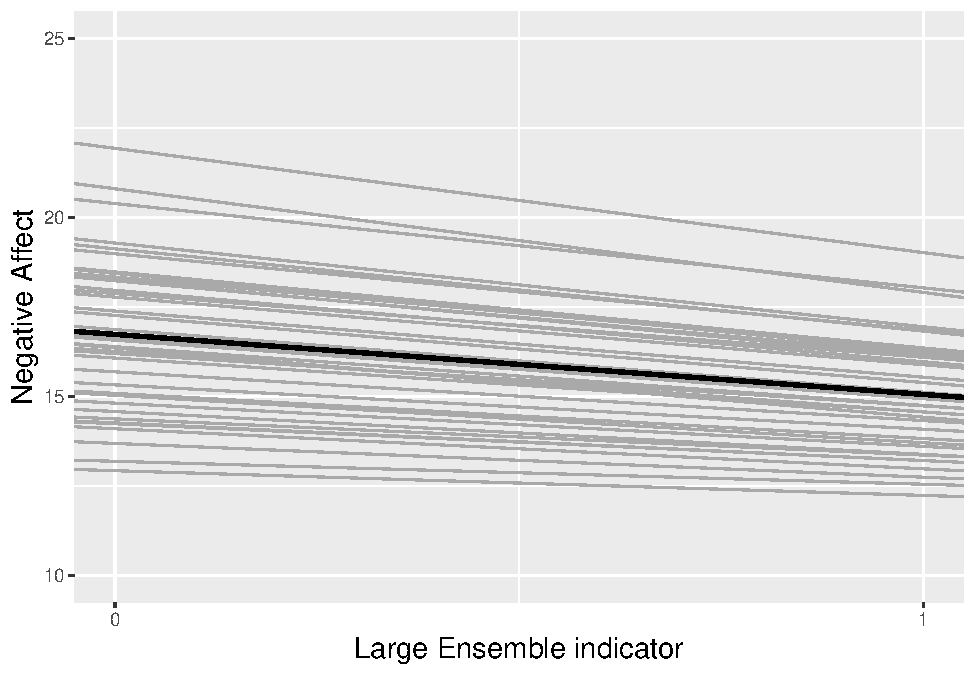
\includegraphics[width=0.6\linewidth]{bookdown-bysh_files/figure-latex/mli-spag1-1} 

}

\caption{The random slopes and intercepts model fitted to the music performance anxiety data.  Each gray line represents one subject, and the thicker black line represents the trend across all subjects.}\label{fig:mli-spag1}
\end{figure}

\begin{figure}

{\centering 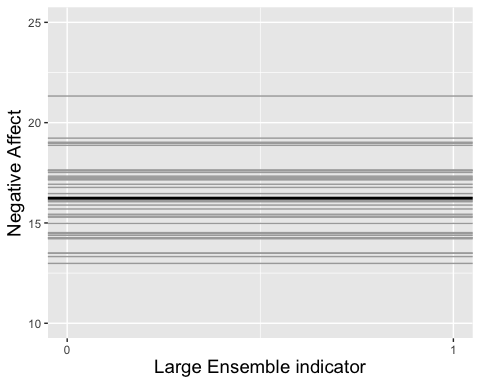
\includegraphics[width=0.6\linewidth]{bookdown-bysh_files/figure-latex/mli-spag0-1} 

}

\caption{The random intercepts model fitted to the music performance anxiety data.  Each gray line represents one subject, and the thicker black line represents the trend across all subjects.}\label{fig:mli-spag0}
\end{figure}

Figures \ref{fig:mli-spag1} and \ref{fig:mli-spag0} use \textbf{empirical Bayes estimates} for the intercepts (\(a_{i}\)) and slopes (\(b_{i}\)) of individual subjects. Empirical Bayes estimates are sometimes called ``shrinkage estimates'' since they combine individual-specific information with information from all subjects, thus ``shrinking'' the individual estimates toward the group averages. Empirical Bayes estimates are often used when a term such as \(a_{i}\) involves both fixed and random components; further detail can be found in \citet{Bryk2002} and \citet{Singer2003}.

\hypertarget{pseudoR2}{%
\subsection{\texorpdfstring{Pseudo \(R^2\) values}{Pseudo R\^{}2 values}}\label{pseudoR2}}

The estimated within-person variance \(\hat{\sigma}^2\) decreased by 3.1\% (from 22.5 to 21.8) from the unconditional means model, implying that only 3.1\% of within-person variability in performance anxiety scores can be explained by performance type. This calculation is considered a \textbf{pseudo R-square} value:
\begin{equation}
\textrm{Pseudo }R^2_{L1} = \frac{\hat{\sigma}^{2}(\textrm{Model A})-\hat{\sigma}^{2}(\textrm{Model B})}{\hat{\sigma}^{2}(\textrm{Model A})} = \frac{22.5-21.8}{22.5} = 0.031
\label{eq:pseudo}
\end{equation}
Values of \(\hat{\sigma}_{u}^{2}\) and \(\hat{\sigma}_{v}^{2}\) cannot be compared to between-person variability from Model A, since the inclusion of performance type has changed the interpretation of these values, although they can provide important benchmarks for evaluating more complex Level Two predictions. Finally, \(\hat{\rho}_{uv}=-0.76\) indicates a strong negative relationship between a subject's performance anxiety before solos and small ensembles and their (typical) decrease in performance anxiety before large ensembles. As might be expected, subjects with higher levels of performance anxiety before solos and small ensembles tend to have smaller increases (or greater decreases) in performance anxiety before large ensembles; those with higher levels of performance anxiety before solos and small ensembles have more opportunity for decreases before large ensembles.

Pseudo \(R^2\) values are not universally reliable as measures of model performance. Because of the complexity of estimating fixed effects and variance components at various levels of a multilevel model, it is not unusual to encounter situations in which covariates in a Level Two equation for, say, the intercept remain constant (while other aspects of the model change), yet the associated pseudo \(R^2\) values differ or are negative. For this reason, pseudo \(R^2\) values in multilevel models should be interpreted cautiously.

\hypertarget{modelc}{%
\subsection{Adding a covariate at Level Two}\label{modelc}}

The initial two-level model described in section \ref{initialmodel} essentially expands upon the random slopes and intercepts model by adding a binary covariate for instrument played at Level Two. We will denote this as Model C:

\begin{itemize}
\item
  Level One:
  \begin{equation}
  Y_{ij} = a_{i}+b_{i}\textstyle{LargeEns}_{ij}+\epsilon_{ij}
  \label{eq:level1modelc}
  \end{equation}
\item
  Level Two:
  \begin{eqnarray*}
  a_{i} & = & \alpha_{0}+\alpha_{1}\textstyle{Orch}_{i}+u_{i} \\
  b_{i} & = & \beta_{0}+\beta_{1}\textstyle{Orch}_{i}+v_{i},
  \end{eqnarray*}
  where \(\epsilon_{ij}\sim N(0,\sigma^2)\) and
  \[ \left[ \begin{array}{c}
            u_{i} \\ v_{i}
          \end{array}  \right] \sim N \left( \left[
          \begin{array}{c}
            0 \\ 0
          \end{array} \right], \left[
          \begin{array}{cc}
            \sigma_{u}^{2} & \\
            \rho\sigma_{u}\sigma_{v} & \sigma_{v}^{2}
          \end{array} \right] \right). \]
\end{itemize}

We found that there are no highly significant fixed effects in Model C (other than the intercept). In particular, we have no significant evidence that musicians playing orchestral instruments reported different performance anxiety scores, on average, for solos and small ensembles than keyboardists and vocalists, no evidence of a difference in performance anxiety by performance type for keyboard players and vocalists, and no evidence of an instrument effect in difference between large ensembles and other types.

Since no terms were added at Level One when expanding from the random slopes and intercepts model (Model B), no discernable changes should occur in explained within-person variability (although small changes could occur due to numerical estimation procedures used in likelihood-based parameter estimates). However, Model C expanded Model B by using the instrument which a subject plays to model both intercepts and slopes at Level Two. We can use pseudo R-square values for both intercepts and slopes to evaluate the impact on between-person variability of adding instrument to Model B.
\begin{equation}
\textrm{Pseudo }R^2_{L2_u} = \frac{\hat{\sigma}_{u}^{2}(\textrm{Model B})-\hat{\sigma}_{u}^{2}(\textrm{Model C})}{\hat{\sigma}_{u}^{2}(\textrm{Model B})} = \frac{6.33-5.66}{6.33} = 0.106
\label{eq:pseudol0}
\end{equation}

\begin{equation}
\textrm{Pseudo }R^2_{L2_v} = \frac{\hat{\sigma}_{v}^{2}(\textrm{Model B})-\hat{\sigma}_{v}^{2}(\textrm{Model C})}{\hat{\sigma}_{v}^{2}(\textrm{Model B})} = \frac{0.74-0.45}{0.74} = 0.392
\label{eq:pseudol1}
\end{equation}
\(\textrm{Pseudo }R^2_{L2_u}\) describes the improvement in Model C over Model B in explaining subject-to-subject variability in intercepts, and \(\textrm{Pseudo }R^2_{L2_v}\) describes the improvement in Model C over Model B in explaining subject-to-subject variability in slopes. Thus, the addition of instrument at Level Two has decreased the between-person variability in mean performance anxiety before solos and small ensembles by 10.6\%, and it has decreased the between-person variability in the effect of large ensembles on performance anxiety by 39.2\%.

We could also run a ``random intercepts'' version of Model C, with no error term in the equation for the slope at Level Two (and thus no covariance between errors at Level Two as well):

\begin{itemize}
\item
  Level One:
  \begin{equation}
  Y_{ij} = a_{i}+b_{i}\textstyle{LargeEns}_{ij}+\epsilon_{ij}
  \label{eq:level1modelcrandint}
  \end{equation}
\item
  Level Two:
  \begin{eqnarray*}
  a_{i} & = & \alpha_{0}+\alpha_{1}\textstyle{Orch}_{i}+u_{i} \\
  b_{i} & = & \beta_{0}+\beta_{1}\textstyle{Orch}_{i},
  \end{eqnarray*}
  where \(\epsilon_{ij}\sim N(0,\sigma^2)\) and \(u_{i}\sim N(0,\sigma_{u}^{2})\).
\end{itemize}

The output below contains REML estimates of our 6 parameters from this simplified version of Model C:

\begin{verbatim}
Formula: na ~ orch + large + orch:large + (1 | id)

Random effects:
 Groups   Name        Variance Std.Dev.
 id       (Intercept)  5.131   2.265   
 Residual             21.882   4.678   
Number of obs: 497, groups:  id, 37

Fixed effects:
            Estimate Std. Error t value
(Intercept)  15.9026     0.6187  25.703
orch          1.7100     0.9131   1.873
large        -0.8918     0.8415  -1.060
orch:large   -1.4650     1.0880  -1.347
\end{verbatim}

\begin{verbatim}
         df      AIC
model.c   8 3002.981
model.c2  6 2999.384
\end{verbatim}

\begin{verbatim}
         df      BIC
model.c   8 3036.650
model.c2  6 3024.635
\end{verbatim}

Note that parameter estimates for the remaining 6 fixed effects and variance components closely mirror the corresponding parameter estimates from Model C. In fact, removing the error term on the slope has improved (reduced) both the AIC and BIC measures of overall model performance. Instead of assuming that the large ensemble effects, after accounting for instrument played, vary by individual, we are assuming that large ensemble effect is fixed across subjects. It is not unusual to run a two-level model like this, with an error term on the intercept equation to account for subject-to-subject differences, but with no error terms on other Level Two equations unless there is an \emph{a priori} reason to allow effects to vary by subject or if the model performs better after building in those additional error terms.

\hypertarget{sec:modeld}{%
\section{Additional covariates: model comparison and interpretability}\label{sec:modeld}}

Recall that we are particularly interested in this study in Level Two covariates---those subject-specific variables that provide insight into why individuals react differently in anxiety-inducing situations. In section \ref{explore}, we saw evidence that subjects with higher baseline levels of negative emotionality tend to have higher performance anxiety levels prior to performances. Thus, in our next step in model building, we will add negative emotionality as a Level Two predictor to Model C. With this addition, our new model can be expressed as a system of Level One and Level Two models:

\begin{itemize}
\item
  Level One:
  \begin{equation}
  Y_{ij} = a_{i}+b_{i}\textstyle{LargeEns}_{ij}+\epsilon_{ij}
  \label{eq:level1modelcnegem}
  \end{equation}
\item
  Level Two:
  \begin{eqnarray*}
  a_{i} & = & \alpha_{0}+\alpha_{1}\textstyle{Orch}_{i}+\alpha_{2}\textstyle{MPQnem}_{i}+u_{i} \\
  b_{i} & = & \beta_{0}+\beta_{1}\textstyle{Orch}_{i}+\beta_{2}\textstyle{MPQnem}_{i}+v_{i},
  \end{eqnarray*}
  or as a composite model:
  \begin{eqnarray*}
  Y_{ij} & = & [\alpha_{0}+\alpha_{1}\textstyle{Orch}_{i}+\alpha_{2}\textstyle{MPQnem}_{i}+\beta_{0}\textstyle{LargeEns}_{ij} \\
   & & \textrm{} + \beta_{1}\textstyle{Orch}_{i}\textstyle{LargeEns}_{ij}+\beta_{2}\textstyle{MPQnem}_{i}\textstyle{LargeEns}_{ij}] \\
   & & \textrm{} + [u_{i}+v_{i}\textstyle{LargeEns}_{ij}+\epsilon_{ij}]
  \end{eqnarray*}
  where error terms are defined as in Model C.
\end{itemize}

From the R output below, we see that, as our exploratory analyses suggested, subjects with higher baseline levels of stress reaction, alienation, and aggression (as measured by the MPQ negative emotionality scale) had significantly higher levels of performance anxiety before solos and small ensembles (t=3.893). They also had somewhat greater differences between large ensembles and other performance types, controlling for instrument (t=-0.575), although this interaction was not statistically significant.

\begin{verbatim}
Formula: na ~ orch + mpqnem + large + orch:large + mpqnem:large + (large |      id)
   Data: music
Random effects:
 Groups   Name        Variance Std.Dev. Corr 
 id       (Intercept)  3.2857  1.8126        
          large        0.5566  0.7461   -0.38
 Residual             21.8114  4.6703        
Number of obs: 497, groups:  id, 37

Fixed effects:
             Estimate Std. Error t value
(Intercept)  11.56801    1.22057   9.478
orch          1.00069    0.81713   1.225
mpqnem        0.14823    0.03808   3.893
large        -0.28018    1.83413  -0.153
orch:large   -0.94927    1.10621  -0.858
mpqnem:large -0.03018    0.05246  -0.575
\end{verbatim}

\hypertarget{interp:modeld}{%
\subsection{Interpretation of parameter estimates}\label{interp:modeld}}

Compared to Model C, the directions of the effects of instrument and performance type are consistent, but the effect sizes and levels of significance are reduced because of the relative importance of the negative emotionality term. Interpretations will also change slightly to acknowledge that we have controlled for a covariate. In addition, interpretations of fixed effects involving negative emotionality must acknowledge that this covariate is a continuous measure and not binary like instrument and performance type:

\begin{itemize}
\tightlist
\item
  \(\hat{\alpha}_{0} = 11.57\). The estimated mean performance anxiety for solos and small ensembles (\texttt{large=0}) is 11.57 for keyboard players and vocalists (\texttt{orch=0}) with negative emotionality of 0 at baseline (\texttt{mpqnem=0}). Since the minimum negative emotionality score in this study was 11, this interpretation, while technically correct, is not practically meaningful.
\item
  \(\hat{\alpha}_{1} = 1.00\). Orchestral instrument players have an estimated mean anxiety level before solos and small ensembles which is 1.00 point higher than keyboardists and vocalists, controlling for the effects of baseline negative emotionality.
\item
  \(\hat{\alpha}_{2} = 0.15\). A one point increase in baseline negative emotionality is associated with an estimated 0.15 mean increase in anxiety levels before solos and small ensembles, after controlling for instrument.
\item
  \(\hat{\beta}_{0} = -0.28\). Keyboard players and vocalists (\texttt{orch=0}) with baseline negative emotionality levels of 0 (\texttt{mpqnem=0}) have an estimated mean decrease in anxiety level of 0.28 points before large ensemble performances compared to other performance types.
\item
  \(\hat{\beta}_{1} = -0.95\). Orchestral instrument players have an estimated mean difference in anxiety levels between large ensembles and other performance types that is 0.95 points lower than the difference for keyboard players and vocalists, controlling for the effects of baseline negative emotionality. For example, orchestral instrumentalists with \texttt{mpqnem=0} have a larger estimated mean decrease in anxiety level of 1.23 points before large ensemble performances, rather than the mean decrease of 0.28 in those who don't play orchestral instruments.
\item
  \(\hat{\beta}_{2} = -0.03\). A one point increase in baseline negative emotionality is associated with an estimated .03 mean decrease in the difference in anxiety levels for large ensembles and other performance types, after controlling for instrument.
\end{itemize}

Some of the detail in these parameter interpretations can be tricky---describing interaction terms, deciding if a covariate must be fixed at 0 or merely held constant, etc. Often it helps to write out models for special cases to isolate the effects of specific fixed effects. We will consider a few parameter estimates from above and see why the interpretations are written as they are.

\begin{itemize}
\item
  \(\hat{\alpha}_{1}\). For solos and small ensembles (\texttt{LargeEns=0}), the following equations describe the fixed effects portion of the composite model for negative affect score for vocalists and keyboardsists (\texttt{Orch=0}) and orchestral instrumentalists (\texttt{Orch=1}):
  \begin{eqnarray*}
  \textstyle{Orch}=0: & & \\
  Y_{ij} & = & \alpha_{0}+\alpha_{2}\textstyle{MPQnem}_{i} \\
  \textstyle{Orch}=1: & & \\
  Y_{ij} & = & (\alpha_{0}+\alpha_{1})+\alpha_{2}\textstyle{MPQnem}_{i}
  \end{eqnarray*}
  Regardless of the subjects' baseline negative emotionality (\texttt{MPQnem}), \(\hat{\alpha}_{1}\) represents the estimated difference in performance anxiety between those playing orchestral instruments and others. This interpretation, however, only holds for solos and small ensembles. For large ensembles, the difference between those playing orchestral instruments and others is actually given by \(\hat{\alpha}_{1}+\hat{\beta}_{1}\), holding \texttt{MPQnem} constant (Show!).
\item
  \(\hat{\beta}_{0}\). Because \texttt{LargeEns} interacts with both \texttt{Orch} and \texttt{MPQnem} in Model C, \(\hat{\beta}_{0}\) only describes the estimated difference between large ensembles and other performance types when both \texttt{Orch=0} and \texttt{MPQnem=0}, thus removing the effects of the interaction terms. If, for instance, \texttt{Orch=1} and \texttt{MPQnem=20}, then the difference between large ensembles and other performance types is given by \(\hat{\beta}_{0}+\hat{\beta}_{1}+20\hat{\beta}_{2}\).
\item
  \(\hat{\beta}_{1}\). As with \(\hat{\alpha}_{1}\), we consider equations describing the fixed effects portion of the composite model for negative affect score for vocalists and keyboardsists (\texttt{Orch=0}) and orchestral instrumentalists (\texttt{Orch=1}), except here we leave \emph{LargeEns} as an unknown rather than restricting the model to solos and small ensembles:
  \begin{eqnarray*}
  \textstyle{Orch}=0: & & \\
  Y_{ij} & = & \alpha_{0}+\alpha_{2}\textstyle{MPQnem}_{i}+\beta_{0}\textstyle{LargeEns}_{ij} \\
   & & \textrm{} +\beta_{2}\textstyle{MPQnem}_{i}\textstyle{LargeEns}_{ij} \\
  \textstyle{Orch}=1: & & \\
  Y_{ij} & = & (\alpha_{0}+\alpha_{1})+\alpha_{2}\textstyle{MPQnem}_{i}+(\beta_{0}+\beta_{1})\textstyle{LargeEns}_{ij} \\
   & & \textrm{} +\beta_{2}\textstyle{MPQnem}_{i}\textstyle{LargeEns}_{ij}
  \end{eqnarray*}
  As long as baseline negative emotionality is held constant (at any level, not just 0), then \(\hat{\beta}_{1}\) represents the estimated difference in the large ensemble effect between those playing orchestral instruments and others.
\end{itemize}

\hypertarget{compare:modeld}{%
\subsection{Model comparisons}\label{compare:modeld}}

At this point, we might ask: do the two extra fixed effects terms in Model D provide a significant improvement over Model C? Nested models such as these can be tested using a likelihood ratio (drop in deviance) test, as we've used in Sections \ref{sec-PoisInference} and \ref{sec-logisticInf} with certain generalized linear models. Since we are comparing models nested in their fixed effects, we use full maximum likelihood methods to estimate model parameters, as discussed in section \ref{multileveltechnical}. As expected, the likelihood is larger (and the log-likelihood is less negative) under the larger model (Model D); our test statistic (14.734) is then -2 times the difference in log-likelihood between Models C and D. Comparing the test statistic to a chi-square distribution with 2 degrees of freedom (signifying the number of additional terms in Model D), we obtain a p-value of .0006. Thus, Model D significantly outperforms Model C.

\begin{Shaded}
\begin{Highlighting}[]
\CommentTok{# anova() automatically uses ML for LRT tests}
\KeywordTok{anova}\NormalTok{(model.d,model.c)}
\end{Highlighting}
\end{Shaded}

\begin{verbatim}
Data: music
Models:
model.c: na ~ orch + large + orch:large + (large | id)
model.d: na ~ orch + mpqnem + large + orch:large + mpqnem:large + (large | 
model.d:     id)
        Df    AIC    BIC  logLik deviance  Chisq Chi Df Pr(>Chisq)    
model.c  8 3007.2 3040.8 -1495.6   2991.2                             
model.d 10 2996.4 3038.5 -1488.2   2976.4 14.734      2  0.0006319 ***
---
Signif. codes:  0 '***' 0.001 '**' 0.01 '*' 0.05 '.' 0.1 ' ' 1
\end{verbatim}

Two models, whether they are nested or not, can be compared using AIC and BIC measures, which were first seen in Chapter \ref{ch-MLRreview} and later used in evaluating generalized linear models. In this case, the AIC clearly favors Model D (2996.7) over Model C (3007.3), whereas the BIC favors Model D (3038.8) only slightly over Model C (3041.0) since the BIC imposes a stiffer penalty on additional terms and additional model complexity. However, the likelihood ratio test is a more reliable method for comparing nested models.

Finally, we note that Model D could be further improved by dropping the negative emotionality by large ensemble interaction term. Not only is the t-value (-0.575) associated with this term of low magnitude, but a likelihood ratio test comparing Model D to a model without \texttt{mpqnem:large} produces an insignificant p-value of 0.5534.

\begin{Shaded}
\begin{Highlighting}[]
\NormalTok{model.d1 <-}\StringTok{ }\KeywordTok{lmer}\NormalTok{(na }\OperatorTok{~}\StringTok{ }\NormalTok{orch }\OperatorTok{+}\StringTok{ }\NormalTok{mpqnem }\OperatorTok{+}\StringTok{ }\NormalTok{large }\OperatorTok{+}\StringTok{ }\NormalTok{orch}\OperatorTok{:}\NormalTok{large }\OperatorTok{+}\StringTok{ }
\StringTok{  }\NormalTok{(large}\OperatorTok{|}\NormalTok{id), }\DataTypeTok{data=}\NormalTok{music)}
\KeywordTok{anova}\NormalTok{(model.d,model.d1)}
\end{Highlighting}
\end{Shaded}

\begin{verbatim}
Data: music
Models:
model.d1: na ~ orch + mpqnem + large + orch:large + (large | id)
model.d: na ~ orch + mpqnem + large + orch:large + mpqnem:large + (large | 
model.d:     id)
         Df    AIC    BIC  logLik deviance  Chisq Chi Df Pr(>Chisq)
model.d1  9 2994.8 3032.7 -1488.4   2976.8                         
model.d  10 2996.4 3038.5 -1488.2   2976.4 0.3513      1     0.5534
\end{verbatim}

\hypertarget{sec:modele}{%
\section{Center covariates}\label{sec:modele}}

As we observed above, the addition of baseline negative emotionality in Model D did not always produce sensible interpretations of fixed effects. It makes no sense to draw conclusions about performance anxiety levels for subjects with MPQNEM scores of 0 at baseline (as in \(\hat{\beta}_{0}\)), since the minimum NEM composite score among subjects in this study was 11. In order to produce more meaningful interpretations of parameter estimates and often more stable parameter estimates, it is often wise to \textbf{center} explanatory variables. Centering involves subtracting a fixed value from each observation, where the fixed value represents a meaningful anchor value (e.g., last grade completed = 12; GPA = 3.0). Often, when there's no pre-defined anchor value, the mean is used to represent a typical case. With this in mind, we can create a new variable
\begin{eqnarray*}
\textstyle{centeredbaselineNEM} = \textstyle{cmpqnem} = \textstyle{mpqnem - mean(mpqnem)} = \textstyle{mpqnem} - 31.63
\end{eqnarray*}
and replace baseline NEM in Model D with its centered version:

\begin{verbatim}
[1] 31.63179
\end{verbatim}

\begin{verbatim}
Formula: na ~ orch + cmpqnem + large + orch:large + cmpqnem:large + (large |      id)
   Data: music
Random effects:
 Groups   Name        Variance Std.Dev. Corr 
 id       (Intercept)  3.2857  1.8126        
          large        0.5566  0.7461   -0.38
 Residual             21.8114  4.6703        
Number of obs: 497, groups:  id, 37

Fixed effects:
              Estimate Std. Error t value
(Intercept)   16.25679    0.54756  29.689
orch           1.00069    0.81713   1.225
cmpqnem        0.14823    0.03808   3.893
large         -1.23484    0.84321  -1.464
orch:large    -0.94927    1.10621  -0.858
cmpqnem:large -0.03018    0.05246  -0.575
\end{verbatim}

As you compare Model D to Model E, you should notice that only two things change -- \(\hat{\alpha}_{0}\) and \(\hat{\beta}_{0}\). All other parameter estimates---both fixed effects and variance components---remain identical; the basic model is essentially unchanged as well as the amount of variability in anxiety levels explained by the model. \(\hat{\alpha}_{0}\) and \(\hat{\beta}_{0}\) are the only two parameter estimates whose interpretations in Model D refer to a specific level of baseline NEM. In fact, the interpretations that held true where \texttt{NEM=0} (which isn't possible) now hold true for \texttt{cmpqnem=0} or when NEM is at its average value of 31.63, which is possible and quite meaningful. Now, parameter estimates using centered baseline NEM in Model E change in value from Model D and produce more useful interpretations:

\begin{itemize}
\tightlist
\item
  \(\hat{\alpha}_{0} = 16.26\). The estimated mean performance anxiety for solos and small ensembles (\texttt{large=0}) is 16.26 for keyboard players and vocalists (\texttt{orch=0}) with an average level of negative emotionality at baseline (\texttt{mpqnem=31.63}).
\item
  \(\hat{\beta}_{0} = -1.23\). Keyboard players and vocalists (\texttt{orch=0}) with an average level of baseline negative emotionality levels (\texttt{mpqnem=31.63}) have an estimated mean decrease in anxiety level of 1.23 points before large ensemble performances compared to other performance types.
\end{itemize}

\hypertarget{modelf}{%
\section{A potential final model for music performance anxiety}\label{modelf}}

We now begin iterating toward a ``final model'' for these data, on which we will base conclusions. Typical features of a ``final multilevel model'' include:

\begin{itemize}
\tightlist
\item
  fixed effects allow one to address primary research questions
\item
  fixed effects control for important covariates at all levels
\item
  potential interactions have been investigated
\item
  variables are centered where interpretations can be enhanced
\item
  important variance components have been included
\item
  unnecessary terms have been removed
\item
  the model tells a ``persuasive story parsimoniously''
\end{itemize}

Although the process of reporting and writing up research results often demands the selection of a sensible final model, it's important to realize that (a) statisticians typically will examine and consider an entire taxonomy of models when formulating conclusions, and (b) different statisticians sometimes select different models as their ``final model'' for the same set of data. Choice of a ``final model'' depends on many factors, such as primary research questions, purpose of modeling, tradeoff between parsimony and quality of fitted model, underlying assumptions, etc. So you should be able to defend any final model you select, but you should not feel pressured to find the one and only ``correct model'', although most good models will lead to similar conclusions.

As we've done in previous sections, we can use (a) t-statistics for individual fixed effects when considering adding a single term to an existing model, (b) likelihood ratio tests for comparing nested models which differ by more than one parameter, and (c) model performance measures such as AIC and BIC to compare non-nested models. Below we offer one possible final model for this data---Model F:

\begin{itemize}
\tightlist
\item
  Level One:
  \begin{equation}
  Y_{ij} = a_{i}+b_{i}\textstyle{previous}_{ij}+c_{i}\textstyle{students}_{ij}+
  d_{i}\textstyle{juried}_{ij}+e_{i}\textstyle{public}_{ij}+f_{i}\textstyle{solo}_{ij}+\epsilon_{ij}
  \label{eq:level1modelf}
  \end{equation}
\item
  Level Two:
  \begin{eqnarray*}
  a_{i} & = & \alpha_{0}+\alpha_{1}\textstyle{mpqpem}_{i}+\alpha_{2}\textstyle{mpqab}_{i} + \alpha_{3}\textstyle{orch}_{i}+\alpha_{4}\textstyle{mpqnem}_{i}+u_{i} \\
  b_{i} & = & \beta_{0}+v_{i}, \\
  c_{i} & = & \gamma_{0}+w_{i}, \\
  d_{i} & = & \delta_{0}+x_{i}, \\
  e_{i} & = & \varepsilon_{0}+y_{i}, \\
  f_{i} & = & \zeta_{0}+\zeta_{1}\textstyle{mpqnem}_{i}+z_{i},
  \end{eqnarray*}
  where \texttt{previous} is the number of previous diary entries filled out by that individual (\texttt{diary-1}); \texttt{students}, \texttt{juried}, and \texttt{public} are indicator variables created from the \texttt{audience} categorical variable (so that ``Instructor'' is the reference level in this model); and, \texttt{solo} is 1 if the performance was a solo and 0 if the performance was either a small or large ensemble.
\end{itemize}

In addition, we assume the following variance-covariance structure at Level Two:

\[ \left[ \begin{array}{c}
            u_{i} \\ v_{i} \\ w_{i} \\ x_{i} \\ y_{i} \\ z_{i}
          \end{array}  \right] \sim N \left( \left[
          \begin{array}{c}
            0 \\ 0 \\ 0 \\ 0 \\ 0 \\ 0
          \end{array} \right], \left[
          \begin{array}{cccccc}
            \sigma_{u}^{2} & & & & & \\
            \sigma_{uv} & \sigma_{v}^{2} & & & & \\
            \sigma_{uw} & \sigma_{vw} & \sigma_{w}^{2} & & & \\
            \sigma_{ux} & \sigma_{vx} & \sigma_{wx} & \sigma_{x}^{2} & & \\
            \sigma_{uy} & \sigma_{vy} & \sigma_{wy} & \sigma_{xy} & \sigma_{y}^{2} & \\
            \sigma_{uz} & \sigma_{vz} & \sigma_{wz} & \sigma_{xz} & \sigma_{yz} & \sigma_{z}^{2}
          \end{array} \right] \right). \]

Being able to write out these mammoth variance-covariance matrices is less important than recognizing the number of variance components that must be estimated by our intended model. In this case, we must use likelihood-based methods to obtain estimates for 6 variance terms and 15 correlation terms at Level Two, along with 1 variance term at Level One. Note that the number of correlation terms is equal to the number of unique pairs among Level Two random effects. In later sections we will consider ways to reduce the number of variance components in cases where the number of terms is exploding or the statistical software is struggling to simultaneously find estimates for all model parameters to maximize the likelihood function.

From the signs of fixed effects estimates in the R output below, we see that performance anxiety is higher when a musician is performing in front of students, a jury, or the general public rather than their instructor, and it is lower for each additional diary the musician previously filled out. In addition, musicians with lower levels of positive emotionality and higher levels of absorption tend to experience greater performance anxiety, and those who play orchestral instruments experience more performance anxiety than those who play keyboards or sing. Addressing the researchers' primary hypothesis, after controlling for all these factors, we have significant evidence that musicians with higher levels of negative emotionality experience higher levels of performance anxiety, and that this association is even more pronounced when musicians are performing solos rather than as part of an ensemble group.

Here are how a couple of key fixed effects would be interpreted in this final model:

\begin{itemize}
\tightlist
\item
  \(\hat{\alpha}_{4} = 0.11\). A one point increase in baseline level of negative emotionality is associated with an estimated 0.11 mean increase in performance anxiety for musicians performing in an ensemble group (\texttt{solo=0}), after controlling for previous diary entries, audience, positive emotionality, absorption, and instrument.
\item
  \(\hat{\zeta}_{1} = 0.08\). When musicians play solos, a one point increase in baseline level of negative emotionality is associated with an estimated 0.19 mean increase in performance anxiety, 0.08 points (73\%) higher than musicians playing in ensemble groups, controlling for the effects of previous diary entries, audience, positive emotionality, absorption, and instrument.
\end{itemize}

\begin{verbatim}
Formula: na ~ previous + students + juried + public + solo + mpqpem +  
    mpqab + orch + mpqnem + mpqnem:solo + (previous + students +      juried + public + solo | id)
   Data: music
Random effects:
 Groups   Name        Variance Std.Dev. Corr                         
 id       (Intercept) 14.16297 3.7634                                
          previous     0.06725 0.2593   -0.69                        
          students     8.28124 2.8777   -0.59  0.07                  
          juried      16.49815 4.0618   -0.58 -0.14  0.79            
          public      12.74352 3.5698   -0.84  0.41  0.59  0.51      
          solo         0.89348 0.9452   -0.66  0.58  0.31  0.02  0.84
 Residual             15.28689 3.9098                                
Number of obs: 497, groups:  id, 37

Fixed effects:
            Estimate Std. Error t value
(Intercept)  8.21678    1.91672   4.287
previous    -0.14280    0.06175  -2.312
students     3.60852    0.77187   4.675
juried       4.06906    1.00548   4.047
public       3.04384    0.89346   3.407
solo         0.57615    1.40604   0.410
mpqpem      -0.08137    0.02426  -3.354
mpqab        0.20435    0.04793   4.264
orch         1.50590    0.58683   2.566
mpqnem       0.11746    0.03599   3.263
solo:mpqnem  0.08015    0.04187   1.915
\end{verbatim}

\hypertarget{multinecessary}{%
\section{Modeling the multilevel structure: is it really necessary?}\label{multinecessary}}

Before going too much further, we should really consider if this multilevel structure has gained us anything over ordinary least squares regression. Sure, multilevel modeling seems more faithful to the inherent structure of the data---performances from the same musician should be more highly correlated than performances from different musicians---but do our conclusions change in a practical sense? Some authors have expressed doubts. For instance Robert Bickel, in his 2007 book, states, ``When comparing OLS and multilevel regression results, we may find that differences among coefficient values are inconsequential, and tests of significance may lead to the same decisions. A great deal of effort seems to have yielded precious little gain'' \citep{Bickel2007}. Others, especially economists, advocate simply accounting for the effect of different Level Two observational units (like \texttt{musicians}) with a sequence of indicator variables for those observational units. We contend that (1) fitting multilevel models is a small extension of OLS regression that is not that difficult to conceptualize and fit, especially with the software available today, and (2) using multilevel models to remain faithful to the data structure can lead to different coefficient estimates and often leads to different (and larger) standard error estimates and thus smaller test statistics. Hopefully you've seen evidence of (1) in this section already; the rest of this section introduces two small examples to help illustrate (2).

\begin{figure}

{\centering 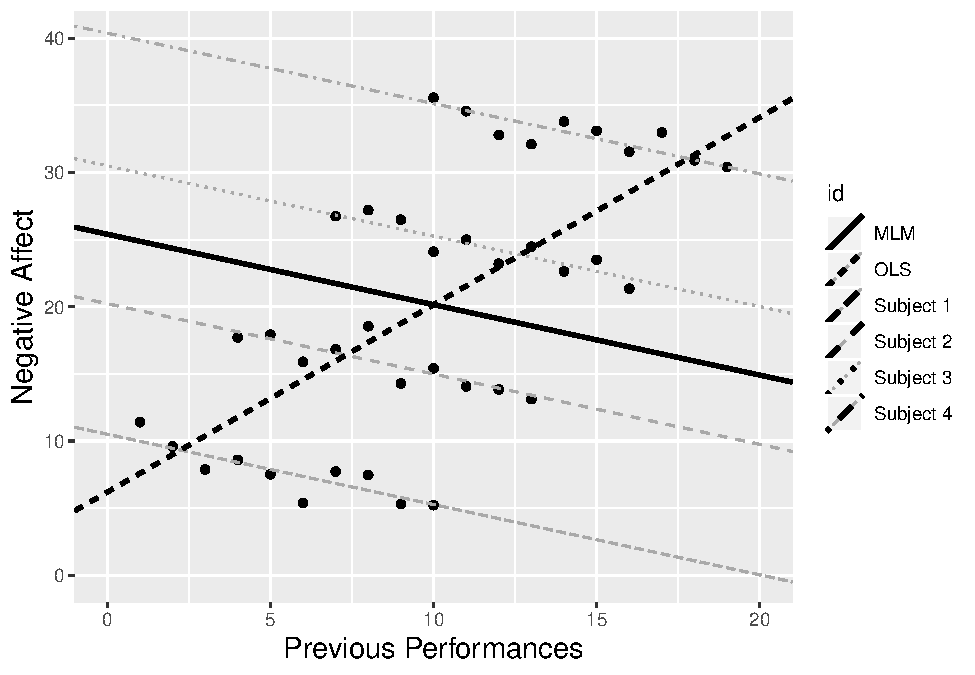
\includegraphics[width=0.6\linewidth]{bookdown-bysh_files/figure-latex/mli-spag2-1} 

}

\caption{Hypothetical data from 4 subjects relating number of previous performances to negative affect.  The solid black line depicts the overall relationship between previous performances and negative affect as determined by a multilevel model, while the dashed black line depicts the overall relationship as determined by an OLS regression model.}\label{fig:mli-spag2}
\end{figure}

Figure \ref{fig:mli-spag2} is based on a simulated data set containing 10 observations from each of 4 subjects. For each subject, the relationship between previous performances and negative affect is linear and negative, with slope approximately -0.5 but different intercepts. The multilevel model (a random intercepts model as described in section \ref{modelb}) shows an overall relationship (the solid black line) that's consistent with the individual subjects---slope around -0.5 with an intercept that appears to average the 4 subjects. Fitting an OLS regression model, however, produces an overall relationship (the dashed black line) that is strongly positive. In this case, by naively fitting the 40 observations as if they were all independent and ignoring subject effects, the OLS regression analysis has gotten the estimated slope of the overall relationship backwards, producing a continuous data version of Simpson's Paradox.



\begin{figure}

{\centering 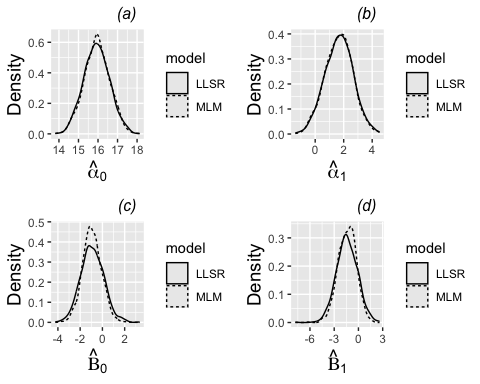
\includegraphics[width=0.6\linewidth]{bookdown-bysh_files/figure-latex/mli-density1-1} 

}

\caption{Density plots of parameter estimates for the four fixed effects of Model C under both a multilevel model and OLS regression. 1000 sets of simulated data for the 37 subjects in our study were produced using estimated fixed and random effects from Model C. For each set of simulated data, estimates of (a) \(\alpha_{0}\), (b) \(\alpha_{1}\), (c) \(\beta_{0}\), and (d) \(\beta_{1}\) were obtained using both a multilevel and an OLS regression model. Each plot then shows a density plot for the 1000 estimates of the corresponding fixed effect using multilevel modeling vs.~a similar density plot for the 1000 estimates using OLS regression.}\label{fig:mli-density1}
\end{figure}



\begin{figure}

{\centering 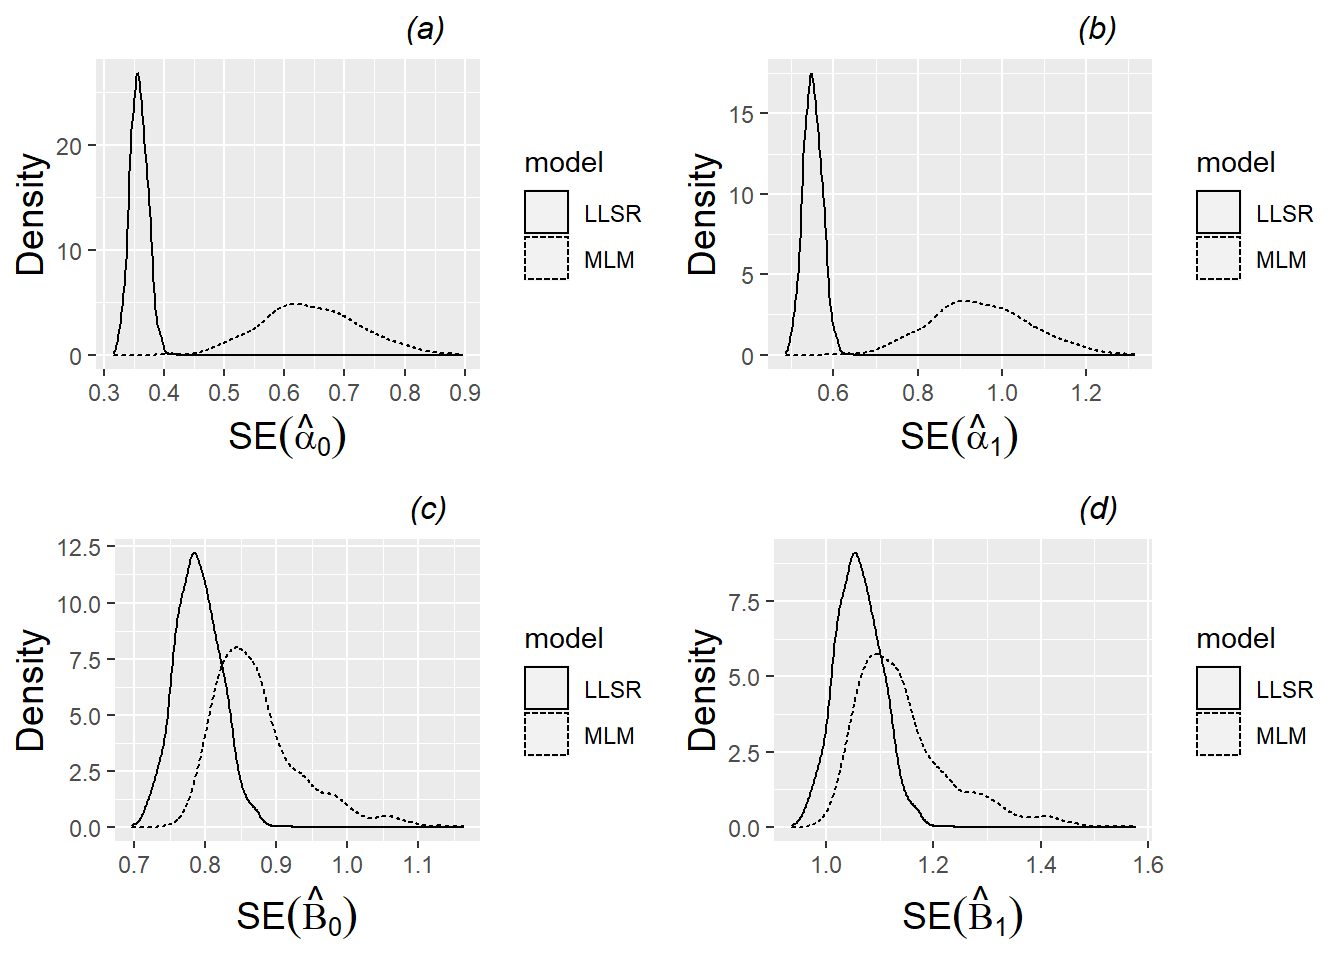
\includegraphics[width=0.6\linewidth]{bookdown-bysh_files/figure-latex/mli-density2-1} 

}

\caption{Density plots of standard errors of parameter estimates for the four fixed effects of Model C under both a multilevel model and OLS regression. 1000 sets of simulated data for the 37 subjects in our study were produced using estimated fixed and random effects from Model C. For each set of simulated data, estimates of (a) SE(\(\alpha_{0}\)), (b) SE(\(\alpha_{1}\)), (c) SE(\(\beta_{0}\)), and (d) SE(\(\beta_{1}\)) were obtained using both a multilevel and an OLS regression model. Each plot then shows a density plot for the 1000 estimates of the corresponding standard error term using multilevel modeling vs.~a similar density plot for the 1000 estimates using OLS regression.}\label{fig:mli-density2}
\end{figure}

Our second example is based upon Model C from section \ref{modelc}, with single binary predictors at both Level One and Level Two. Using the estimated fixed effects coefficients and variance components from random effects produced in Model C, we generated 1000 sets of simulated data. Each set of simulated data contained 497 observations from 37 subjects just like the original data, with relationships between negative affect and large ensembles and orchestral instruments (along with associated variability) governed by the estimated parameters from Model C. Each set of simulated data was used to fit both a multilevel model and an OLS regression model, and the estimated fixed effects (\(\hat{\alpha}_{0}\), \(\hat{\alpha}_{1}\), \(\hat{\beta}_{0}\), and \(\hat{\beta}_{1}\)) and their standard errors were saved. Figure \ref{fig:mli-density1} shows density plots comparing the 1000 estimated fixed effects for each fixed effect from the two modeling approaches; in general, estimates from multilevel modeling and OLS regression tend to agree pretty well, without noticeable bias. Based on coefficient estimates alone, there appears to be no reason to favor multilevel modeling over OLS regression in this example, but Figure \ref{fig:mli-density2} tells a different story. Figure \ref{fig:mli-density2} shows density plots comparing the 1000 estimated standard errors associated with each fixed effect from the two modeling approaches; in general, standard errors are markedly larger with multilevel modeling than OLS regression. This is not unusual, since OLS regression assumes all 497 observations are independent while multilevel modeling acknowledges that, with correlated data within subject, there are fewer than 497 independent pieces of data. Therefore, OLS regression can overstate precision, producing t-statistics for each fixed effect that tend to be larger than they should be; the number of significant results in OLS regression are then not reflective of the true structure of the data.

\hypertarget{notesr8}{%
\section{Notes on Using R (Optional)}\label{notesr8}}

Initial examination of the data for Case Study \ref{cs:music} shows a couple of features that must be noted. First, there are 37 unique study participants, but they are not numbered successively from 1 to 43. The majority of participants filled out 15 diaries, but several filled out fewer (with a minimum of 2); as with participant IDs, diary numbers within participant are not always successively numbered. Finally, missing data is not an issue in this data set, since researchers had already removed participants with only 1 diary entry and performances for which the type was not recorded (of which there were 11).

The R code below runs the initial multilevel model in section \ref{initialmodel}. Multilevel model notation in R is based on the composite model formulation. Here, the response variable is \texttt{na}, while \texttt{orch}, \texttt{large}, and \texttt{orch:large} represent the fixed effects \(\alpha_{1}\), \(\beta_{0}\), and \(\beta_{1}\), along with the intercept \(\alpha_{0}\) which is included automatically. Note that a colon is used to denote an interaction between two variables. Error terms and their associated variance components are specified in \texttt{(large\textbar{}id)}, which is equivalent to \texttt{(1+large\textbar{}id)}. This specifies two error terms at Level Two (the \texttt{id} level): one corresponding to the intercept (\(u_{i}\)) and one corresponding to the large ensemble effect (\(v_{i}\)); the multilevel model will then automatically include a variance for each error term in addition to the covariance between the two error terms. A variance associated with a Level One error term is also automatically included in the multilevel model. Note that there are ways to override the automatic inclusion of certain variance components; for example, \texttt{(0+large\textbar{}id)} would not include an error term for the intercept (and therefore no covariance term at Level Two either).

\begin{Shaded}
\begin{Highlighting}[]
\NormalTok{model0 <-}\StringTok{ }\KeywordTok{lmer}\NormalTok{(na }\OperatorTok{~}\StringTok{ }\NormalTok{orch }\OperatorTok{+}\StringTok{ }\NormalTok{large }\OperatorTok{+}\StringTok{ }\NormalTok{orch}\OperatorTok{:}\NormalTok{large }\OperatorTok{+}
\StringTok{  }\NormalTok{(large}\OperatorTok{|}\NormalTok{id), }\DataTypeTok{REML=}\NormalTok{T, }\DataTypeTok{data=}\NormalTok{music)}
\KeywordTok{summary}\NormalTok{(model0)}
\end{Highlighting}
\end{Shaded}

\hypertarget{exercises-7}{%
\section{Exercises}\label{exercises-7}}

\hypertarget{conceptual-exercises-5}{%
\subsection{Conceptual Exercises}\label{conceptual-exercises-5}}

\begin{enumerate}
\def\labelenumi{\arabic{enumi}.}
\item
  \textbf{Housing Prices.} \citet{Brown2004} describe ``A Hierarchical Linear Model Approach for Assessing the Effects of House and Neighborhood Characteristics on Housing Prices''. Based on the title of their paper: (a) give the observational units at Level One and Level Two, and (b) list potential explanatory variables at both Level One and Level Two.
\item
  In the preceding problem, why can't we assume all houses in the data set are independent? What would be the potential implications to our analysis of assuming independence among houses?
\item
  In the preceding problem, for each of the following sets of predictors: (a) write out the two-level model for predicting housing prices, (b) write out the corresponding composite model, and (c) determine how many model parameters (fixed effects and variance components) must be estimated.

  \begin{itemize}
  \tightlist
  \item
    Square footage, number of bedrooms
  \item
    Median neighborhood income, rating of neighborhood schools
  \item
    Square footage, number of bedrooms, age of house, median neighborhood housing price
  \item
    Square footage, median neighborhood income, rating of neighborhood schools, median neighborhood housing price
  \end{itemize}
\item
  \textbf{Music Performance Anxiety.} Describe a situation in which the two plots in Figure \ref{fig:mli-boxmat1} might tell different stories.
\item
  Explain the difference between \(a_{i}\) in Equation \eqref{eq:level2s0} and \(\hat{a}_{i}\) in Equation \eqref{eq:level2s0hat}.
\item
  Why is the contour plot for multivariate normal density in Figure \ref{fig:contour-boundary} (b) tilted from southwest to northeast, but the contour plot in Figure \ref{fig:contour-boundary} (a) is not tilted?
\item
  In Table \ref{tab:table3chp8}, note that the standard errors associated with estimated coefficients under independence are lower than standard errors under alternative analysis methods. Why is that often the case?
\item
  Why is Model A (Section \ref{modela}) sometimes called the ``unconditional means model''? Why is it also sometimes called the ``random intercepts model''? Are these two labels consistent with each other?
\item
  Consider adding an indicator variable in Model B (Section \ref{randomslopeandint}) for Small Ensemble performances.

  \begin{itemize}
  \tightlist
  \item
    Write out the two-level model for performance anxiety,
  \item
    Write out the corresponding composite model,
  \item
    Determine how many model parameters (fixed effects and variance components) must be estimated, and
  \item
    Explain how the interpretation for the coefficient in front of Large Ensembles would change.
  \end{itemize}
\item
  Give a short rule in your own words describing when an interpretation of an estimated coefficient should ``hold constant'' another covariate or ``set to 0'' that covariate (see Section \ref{interp:modeld}).
\item
  The interpretation of \(\hat{\alpha}_{0}\) in Section \ref{interp:modeld} claims that ``This interpretation, however, only holds for solos and small ensembles. For large ensembles, the difference between those playing orchestral instruments and others is actually given by \(\hat{\alpha}_{1}+\hat{\beta}_{1}\), holding MPQNEM constant.'' Show that this claim is true.
\item
  Explain how the interpretations of the following parameter estimates change (or don't change) as we change our model:

  \begin{itemize}
  \tightlist
  \item
    \(\hat{\alpha}_{0}\) from Model A to B to C to D to E
  \item
    \(\hat{\beta}_{1}\) from Model B to C to D to E
  \item
    \(\hat{\alpha}_{1}\) from Model C to D to E
  \item
    \(\hat{\beta}_{1}\) from Model C to D to E
  \item
    \(\hat{\sigma}_{u}\) from Model A to B to C to D to E
  \item
    \(\hat{\sigma}_{v}\) from Model B to C to D to E
  \end{itemize}
\item
  When moving from Model B to Model C in Section \ref{modelc}, \(\hat{\sigma}_{u}^{2}\) increases slightly. Why might this have occurred?
\item
  Interpret other estimated parameters from Model F beyond those interpreted in Section \ref{modelf}: \(\hat{\alpha}_{0}\), \(\hat{\alpha}_{2}\), \(\hat{\alpha}_{3}\), \(\hat{\beta}_{0}\), \(\hat{\gamma}_{0}\), \(\hat{\zeta}_{0}\), \(\hat{\rho}_{wx}\), \(\hat{\sigma}^{2}\), \(\hat{\sigma}_{u}^{2}\), and \(\hat{\sigma}_{z}^{2}\).
\item
  Explain Figure \ref{fig:mli-spag2} in your own words. Why would OLS regression produce a misleading analysis in this case, but multilevel models would not?
\item
  Summarize Figures \ref{fig:mli-density1} and \ref{fig:mli-density2} in your own words.
\end{enumerate}

\hypertarget{guided-exercise-1}{%
\subsection{Guided Exercise}\label{guided-exercise-1}}

\begin{enumerate}
\def\labelenumi{\arabic{enumi}.}
\item
  \textbf{Music Performance Joy.} In this chapter, we studied models for predicting music performance anxiety, as measured by the negative affect scale from the PANAS instrument. Now we will examine models for predicting the happiness of musicians prior to performances, as measured by the positive affect scale from the PANAS instrument.

  To begin, run the following models:

  \begin{itemize}
  \tightlist
  \item
    Model A = unconditional means model
  \item
    Model B = indicator for instructor audience type and indicator for student audience type at Level One;
    no Level Two predictors
  \item
    Model C = indicator for instructor audience type and indicator for student audience type at Level One;
    centered MPQ absorption subscale as Level Two predictor for intercept and all slope terms
  \item
    Model D = indicator for instructor audience type and indicator for student audience type at Level One;
    centered MPQ absorption subscale and a male indicator as Level Two predictors for intercept and all slope terms
  \end{itemize}

  \begin{enumerate}
  \def\labelenumii{\arabic{enumii}.}
  \tightlist
  \item
    Perform an exploratory data analysis by comparing positive affect (happiness) to Level One and Level Two covariates using appropriate graphs. Comment on interesting trends, supporting your comments with appropriate summary statistics.
  \item
    Report estimated fixed effects and variance components from Model A, using proper notation from this section (no interpretations required). Also report and interpret an intraclass correlation coefficient.
  \item
    Report estimated fixed effects and variance components from Model B, using proper notation from this section. Interpret your MLE estimates for \(\hat{\alpha}_{0}\) (the intercept), \(\hat{\beta}_{1}\) (the instructor indicator), and \(\hat{\sigma}_{u}\) (the Level Two standard deviation for the intercept). Also report and interpret an appropriate pseudo-Rsquare value.
  \item
    Write out Model C, using both separate Level One and Level Two models as well as a composite model. Be sure to express distributions for error terms. How many parameters must be estimated in Model C?
  \item
    Report and interpret the following parameter estimates from Model C: \(\hat{\alpha}_{0}\), \(\hat{\alpha}_{1}\), \(\hat{\gamma}_{0}\), \(\hat{\beta}_{1}\), \(\hat{\sigma}_{u}\), \(\hat{\sigma}_{v}\), and \(\hat{\rho}_{uv}\). Interpretations for variance components should be done in terms of standard deviations and correlation coefficients.
  \item
    Report and interpret the same parameter estimates listed above from Model D. In each case, the new interpretation should involve a small modification of your interpretation from Model C. Use underlines or highlights to denote the part of the Model D interpretation that differs from the Model C interpretation.
  \item
    Also report and interpret the following parameter estimates from Model D: \(\hat{\alpha}_{2}\) and \(\hat{\beta}_{2}\).
  \item
    Use a deviance statistic (likelihood ratio test) to compare Model C vs.~Model D. Give a test statistic and p-value, then state a conclusion. Also compare Models C and D with appropriate pseudo-Rsquare value(s) and with AIC and BIC statistics.
  \end{enumerate}
\end{enumerate}

\hypertarget{open-ended-exercises-3}{%
\subsection{Open-ended Exercises}\label{open-ended-exercises-3}}

\begin{enumerate}
\def\labelenumi{\arabic{enumi}.}
\item
  \textbf{Political Ambiguity.} \citet{Chapp2018} explored 2014 congressional candidates' ambiguity on political issues in their paper, \emph{Going Vague: Ambiguity and Avoidance in Online Political Messaging}. They hand coded a random sample of 2012 congressional candidates' websites, assigning an ambiguity score. 2014 websites were then automatically scored using Wordscores, a program designed for political textual analysis. In their paper, they fit a multilevel model of candidates' ambiguities with predictors at both the candidate and district levels. Some of their hypotheses include that:

  \begin{itemize}
  \tightlist
  \item
    ``when incumbents do hazard issue statements, these statements will be marked by a higher degree of clarity.'' (Hypothesis 1b)\\
  \item
    ``ideological distance will be associated with greater ambiguity.'' (Hypothesis 2a)\\
  \item
    ``controlling for ideological distance, ideological extremity should correspond to less ambiguity.'' (Hypothesis 2b)
  \item
    ``more variance in attitudes will correspond to a higher degree of ambiguity in rhetoric'' (Hypothesis 3a)
  \item
    ``a more heterogeneous mix of subgroups will also correspond to a higher degree of ambiguity in rhetoric'' (Hypothesis 3b)
  \end{itemize}

  Their data can be found in \texttt{ambiguity.csv}. Variables of interest include:

  \begin{itemize}
  \tightlist
  \item
    \texttt{ambiguity} = assigned ambiguity score. Higher scores indicate greater clarity (less ambiguity)\\
  \item
    \texttt{democrat} = 1 if a Democrat, 0 otherwise (Republican)
  \item
    \texttt{incumbent} = 1 if an incumbent, 0 otherwise
  \item
    \texttt{ideology} = a measure of the candidate's left-right orientation. Higher (positive) scores indicate more conservative candidates and lower (negative) scores indiciate more liberal candidates.
  \item
    \texttt{mismatch} = the distance between the candidate's ideology and the district's ideology (candidate ideology scores were regressed against district ideology scores; mismatch values represent the absolute value of the residual associated with each candidate)
  \item
    \texttt{distID} = the congressional district's unique ID
  \item
    \texttt{distLean} = the district's political leaning. Higher scores imply more conservative districts.
  \item
    \texttt{attHeterogeneity} = a measure of the variability of ideologies within the district. Higher scores imply more attitidunal heterogeneity among voters.
  \item
    \texttt{demHeterogeneity} = a measure of the demographic variability within the district. Higher scores imply more demographic heterogeneity among voters.

    With this in mind, fit your own models to address these hypotheses from \citet{Chapp2018}. Be sure to use a two level structure to account for variables at both the candidate and district levels.\\
  \end{itemize}
\item
  \textbf{Airbnb in Chicago.} \citet{Trinh2018} collected data on 1561 Airbnb listings in Chicago from August 2016, and then they merged in information from the neighborhood (out of 43 in Chicago) where the listing was located. We can examine traits that are associated with listings that command a higher price. Conduct an EDA, build a multilevel model, and interpret model coefficients to answer questions such as: What are characteristics of a higher priced listing? Are the most influential traits associated with individual listings or entire neighborhoods? Are there intriguing interactions where the effect of one variable depends on levels of another?
\end{enumerate}

The following variables can be found in \texttt{airbnb.csv} or derived from the variables found there:

\begin{itemize}
\tightlist
\item
  \texttt{overall\_satisfaction} = rating on a 0-5 scale.\\
\item
  \texttt{satisfaction} = 1 if \texttt{overall\_satisfaction} is 5, 0 otherwise
\item
  \texttt{price} = price for one night (in dollars)
\item
  \texttt{reviews} = number of reviews posted
\item
  \texttt{room\_type} = Entire home/apt, Private room, or Shared room
\item
  \texttt{accommodates} = number of people the unit can hold
\item
  \texttt{bedrooms} = number of bedrooms
\item
  \texttt{minstay} = minimum length of stay (in days)
\item
  \texttt{neighborhood} = neighborhood where unit is located (1 of 43)
\item
  \texttt{district} = district where unit is located (1 of 9)
\item
  \texttt{WalkScore} = quality of the neighborhood for walking (0-100)
\item
  \texttt{TransitScore} = quality of the neighborhood for public transit (0-100)
\item
  \texttt{BikeScore} = quality of the neighborhood for biking (0-100)
\item
  \texttt{PctBlack} = proportion of black residents in a neighborhood
\item
  \texttt{HighBlack} = 1 if \texttt{PctBlack} above .60, 0 otherwise
\end{itemize}

\begin{enumerate}
\def\labelenumi{\arabic{enumi}.}
\setcounter{enumi}{2}
\item
  \textbf{Project 5183.} The Colorado Rockies, a Major League Baseball team, instigated a radical experiment on June 20th, 2012. Hopelessly out of contention for the playoffs and struggling again with their pitching, the Rockies decided to limit their starting pitchers to 75 pitches from June 20th until the end of the year with the hope of improving a struggling starting rotation, teaching pitchers how to pitch to contact (which results in low pitch counts), and at the same time trying to conserve young arms. Data has shown that, as a game progresses, fatigue becomes a big factor in a pitcher's performance; if a pitcher has to tweak his mechanics to try to make up for a fatigued body, injuries can often occur. In addition, pitchers often struggle as they begin facing the same batters over again later in games. The Rockies called their experiment ``Project 5183'' to acknowledge the altitude at Coors Field, their home ballpark, and the havoc that high altitude can wreak on pitchers.

  A team of students collected 2012 data on Rockies pitchers from FanGraphs to evaluate Project 5183. \citep{Strutz2013} In a successful experiment, Colorado pitchers on a strict limit of 75 pitches would throw more strikes and yet record fewer strikeouts (pitching to contact rather than taking more pitches to attempt to strike batters out). Different theories explain whether these pitchers would throw harder (since they don't have to save themselves) or throw slower (in order to throw more strikes). But the end result the Rockies hoped to observe was that their pitchers pitch better (allow fewer runs to the opponent) with a pitch limit.

  The data set \texttt{FinalRockiesdata.csv} contains information for 7 starting pitchers who started at least one game before June 20th (without a pitch limit) and at least one game after June 20th (with a limit of 75 pitches). Key response variables include:

  \begin{itemize}
  \tightlist
  \item
    \texttt{vFA} = average fastball velocity
  \item
    \texttt{K.9} = strikeouts per nine innings
  \item
    \texttt{ERA} = earned runs per nine innings
  \item
    \texttt{Pitpct} = percentage of strikes thrown
  \end{itemize}

  The primary explanatory variable of interest is \texttt{PCL} (an indicator variable for if a pitch count limit is in effect). Other potential confounding variables that may be important to control for include \texttt{Coors} (whether or not the game was played in Coors Field, where more runs are often scored because of the high altitude and thin air) and \texttt{Age} of the pitcher.

  Write a short report summarizing the results of Project 5183. (You may notice a few variance components with unusual estimates, such as an estimated variance of 0 or an estimated correlation of 1. These estimates have encountered boundary constraints; we will learn how to deal with these situations in Section \ref{sec:boundary}. For now ignore these variance components; the fixed effects coefficients are still reliable and their interpretations valid.)
\end{enumerate}

  \bibliography{bib/articles.bib,bib/books.bib,bib/misc.bib}

\end{document}
